\documentclass[class=article, crop=false, 12pt]{standalone}
\usepackage[subpreambles=true]{standalone}
\usepackage{../.common/common}


\author{Tony Shing}
%\pretitle{Supplementary}

\topic{T14A (Electromagnetism)}
\title{Magnetic Induction}

\version{2025} % leave blank for omitting

\begin{document}

\maketitle


\begin{overview}
    \begin{itemize}
        \item Motion under Lorentz force
        \item Faraday's law: Motional \& transformer EMF
        \item Lenz's law: Direction of induced EMF
        \item Appendix: A brief history of electromagnetism
    \end{itemize}
\end{overview}

\vskip 1em
In electromagnetism, 
theoretically every problem can be solved through a set of PDEs
called the \bf{Maxwell Equations}.\\[-2em]
\begin{center}
    \begin{minipage}{0.3\textwidth}
        \aleq{
            \div \vvec{E} &= \frac{\rho}{\epsilon_0}\\
            \tkn{maxwell_faraday}{\curl} \vvec{E} &= -\pdvv{\vvec{B}}{t}
        }
    \end{minipage}
    \hspace{0.05\textwidth}
    \begin{minipage}{0.3\textwidth}
        \aleq{
            \div \vvec{B} &= 0\\
            \curl \vvec{B} &= \mu_0 \vvec{J} + \mu_0\epsilon_0\pdvv{\vvec{E}}{t}
        }
    \end{minipage}
\end{center}
\addArrow[blue]{maxwell_faraday}{(-5ex,0)}{}{(-3ex,1ex)}

However, a \it{system of PDEs} is too complicated to be solved.
So we need to learn different "tricks" to avoid them,
which are enough for some simple scenarios.\\

Magnetic induction concerns the \nth{3} equation of the set - \cul[blue]{Faraday's law}. 





\linesep
% content begins here
% Section %%%%%%%%%%%%%%%%%%%%%%%%%%%%%%%%%%%%%%%%%%%%%%%%%%%%
\section{Motion under Lorentz Force}

Nowadays we know that Lorentz force is the fundamental explanation to magnetic induction.
But interestingly, it was formulated correctly only in the very late history of classical E\&M.
\aleq{
    \vvec{F} &= \vvec{F}_E + \vvec{F}_B \\
    \Aboxed{
        &= q\vvec{E} + q\vvec{v}\cross\vvec{B}
    }
}

In general, $\vvec{E}$ and $\vvec{B}$ can be functions of time and position,
but here we will only discuss \cul[red]{the special case when the fields are constant}.\\

By symmetry, we can assume that $\vvec{B}$ is only in $\hhat{z}$ direction, 
i.e. $\vvec{B} = B_z\hhat{z}$.
Then the Newton's \nth{2} law can be expanded as
\aleq{
    m\vvec{a} = m\dvv{t}\bmat{v_x\\v_y\\v_z} = q\bmat{E_x\\E_y\\E_z} 
        + q\bdet{\hhat{x} & \hhat{y} & \hhat{z}\\ v_x & v_y & v_z \\ 0 & 0 & B_z}
}

which is a system of 3 first order linear ODEs.
\aleq{
    \bcase{
        m\dvv{v_x}{t} &= qE_x + qv_yB_z\\
        m\dvv{v_y}{t} &= qE_y - qv_xB_z\\
        m\dvv{v_z}{t} &= qE_z
    }
}

This system is simple enough that we do not need to use any matrix methods.
\begin{itemize}
    \item \bf{\ul{Equation for z component}}\\[0.5ex]
    Motion in $z$ direction is independent of $x$/$y$.
    It can be solved alone.
    \aleq{
        m\dvv{v_z}{t} = qE_z 
        \qquad\Rightarrow\qquad
        v_z(t) &= \frac{qE_z}{m}t + v_{z0}\\[1em]
        \qquad\Rightarrow\qquad
        z(t) &= \half\frac{qE_z}{m}t^2 
            + \tkn{init_vz}{\cul[blue]{v_{z0}}}t + \tkn{init_z}{\cul[blue]{z_0}}
    }
    \addArrow[blue]{init_vz}{(-1ex,-2ex)}{\scriptsize Initial\\[-1ex]\scriptsize z velocity}{(0,-1ex)}{(-2ex,-1ex)}
    \addArrow[blue]{init_z}{(1ex,-2ex)}{\scriptsize Initial\\[-1ex]\scriptsize z coordinate}{(0,-1ex)}{(2ex,-1ex)}
    
    \vskip 1ex
    which is just a constant acceleration motion with an acceleration $\dfrac{qE_z}{m}$.

    \item \bf{\ul{Equation for x/y components}}\\[0.5ex]
    They can be solved by first differentiating one of them,
    then substitute into the other.
    \aleq{
        \dvv[2]{v_x}{t} &= \frac{qB_z}{m}\dvv{v_y}{t} \\[1ex]
        &= \frac{qB_z}{m}\qty(\frac{qE_y}{m}-\frac{qB_z}{m}v_x)\\[1ex]
        &= - \frac{q^2B_z^2}{m}\qty(v_x - \frac{E_y}{B_z})
    }

    which is the familiar ODE of SHM.
    \aleq{
        v_x(t) &= -C \sin\qty(\frac{qB_z}{m}t + \phi) + \frac{E_y}{B_z}\\[1ex]
        \Rightarrow\quad x(t) &= \cub[red]{C\qty(\frac{m}{qB_z})}{\text{A constant}}\cos \qty(\frac{qB_z}{m}t + \phi) 
            + \frac{E_y}{B_z}t + x_0\\[1ex]
        &= \tkn{init_r}{\cul[blue]{R}} \cos \qty(\frac{qB_z}{m}t + \tkn{phase}{\cul[blue]{\phi}}) 
            + \frac{E_y}{B_z}t + \tkn{init_x}{\cul[blue]{x_0}}
    }
    \addArrow[red]{init_r}{(5ex,4ex)}{}{(1ex,2ex)}
    \addArrow[blue]{init_r}{(0,-4ex)}{\scriptsize Radius}{(0,-1ex)}
    \addArrow[blue]{phase}{(0,-4ex)}{\scriptsize Phase}{(0,-1ex)}
    \addArrow[blue]{init_x}{(0,-3ex)}{\scriptsize Initial\\[-1ex]\scriptsize x coordinate}{(0,-1ex)}{(0,-1ex)}

    \vskip 1em
    And subsitute back to equation of $v_y$ gives
    \aleq{
        v_y(t) &= \frac{m}{qB_z}\dvv{v_x}{t} - \frac{E_x}{B_z}
        = -C \cos\qty(\frac{qB_z}{m}t + \phi) - \frac{E_x}{B_z}\\[1ex]
        \Rightarrow\quad y(t) &= -\cub[red]{C \qty(\frac{m}{qB_z})}{\text{A constant}} \sin \qty(\frac{qB_z}{m}t + \phi) 
            - \frac{E_x}{B_z}t + y_0 \\[1ex]
        &= -\tkn{init_r2}{\cul[blue]{R}} \sin \qty(\frac{qB_z}{m}t + \tkn{phase2}{\cul[blue]{\phi}}) 
            - \frac{E_y}{B_z}t + \tkn{init_y}{\cul[blue]{x_0}}
    }
    \addArrow[red]{init_r2}{(5ex,4ex)}{}{(1ex,2ex)}
    \addArrow[blue]{init_r2}{(0,-4ex)}{\scriptsize Radius}{(0,-1ex)}
    \addArrow[blue]{phase2}{(0,-4ex)}{\scriptsize Phase}{(0,-1ex)}
    \addArrow[blue]{init_y}{(0,-3ex)}{\scriptsize Initial\\[-1ex]\scriptsize y coordinate}{(0,-1ex)}{(0,-1ex)}

    \vskip 1em
    The result $x$/$y$ motion is a combination of circular motion + drifting.

    \begin{center}
        \begin{minipage}{0.5\linewidth}
            \centering
            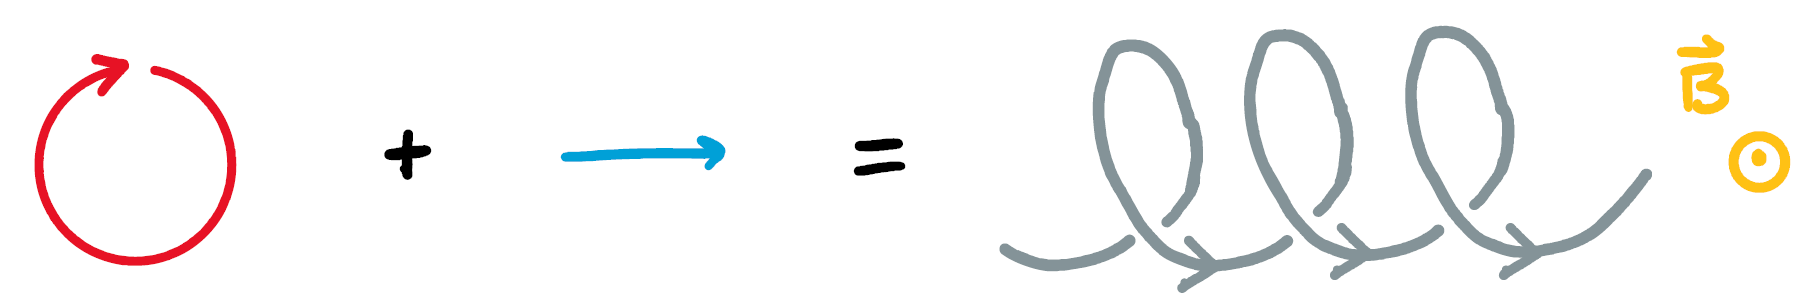
\includegraphics[width=\textwidth]{lorentz}
        \end{minipage}
    \end{center}

    \vskip -2ex
    \aleq{
        \bmat{x(t)\\y(t)} 
        = 
        \cus[red]{R\bmat{\cos \qty(\frac{qB_z}{m}t+\phi) \\ -\sin \qty(\frac{qB_z}{m}t+\phi)}}{\text{Circular motion}}
        \ +\ \cus[blue]{\inv{B_z}\bmat{E_y\\-E_x}t}{\text{Drifting}} \ +\ \bmat{x_0\\y_0}
    }

    \begin{enumerate}
        \item Be careful that the drifting direction is not intuitive: 
        \begin{itemize}
            \item With $E_x$ only, drifting direction = $-\hhat{y}$
            \item With $E_y$ only, drifting direction = $\hhat{x}$
        \end{itemize}
        In general, the drifting is along the direction of $\vvec{E}\cross\vvec{B}$ 
        with a speed $\dfrac{\norm{\vvec{E}}}{\norm{\vvec{B}}}$.
    
        \vskip 1em
        \item The rotation radius and speed maintain a constant ratio:
        \aleq{
            \text{Radius}=R \qquad\Rightarrow\qquad \text{Speed}=\frac{qB_z}{m}R
        }
        i.e. Angular velocity is always $\omega = \dfrac{qB_z}{m}$,
        independent of the charge's initial velocity.
        You can also arrive at the same result from equation of circular motion:
        \aleq{
            \frac{mv^2}{R} &= qvB \\
            v &= \frac{qB}{m}R
        }
        (But how do you argue that it is a circular motion without solving ODEs?)

    \end{enumerate}
\end{itemize}






\linesep
% Section %%%%%%%%%%%%%%%%%%%%%%%%%%%%%%%%%%%%%%%%%%%%%%%%%%%%
\section{The Theory of Magnetic Induction}


%%%%%%%%%%%%%%
\subsection{EMF - Force or Voltage?}

The term \bf{electromotive force} (EMF) was invented by 
\href{https://en.wikipedia.org/wiki/Alessandro_Volta}{Alessandro Volta} in 1801,
for explaining observations in electrochemistry.

\begin{center}
    \begin{minipage}{0.2\linewidth}
        \centering
        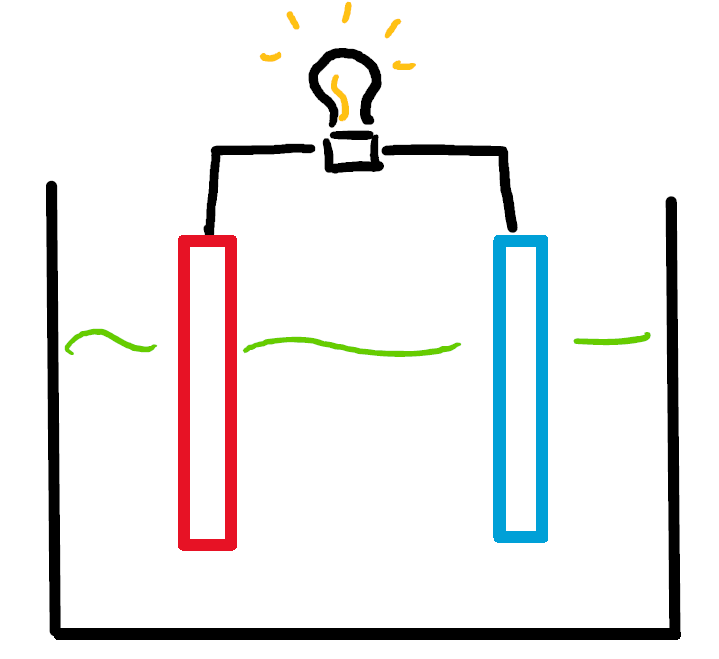
\includegraphics[width=\textwidth]{electrolyte}
    \end{minipage}
    \hspace{0.01\textwidth}
        \begin{minipage}{0.55\linewidth}
            \begin{itemize}
            \item[$\Rightarrow$] Current generates spontaneously.
            \item[$\Rightarrow$] There must be some "force" reponsible for it! 
        \end{itemize}
    \end{minipage}
\end{center}

In early 1800s, scientists tended to describe things like a mechanical system,
i.e. any motions of objects must be driven by some kind of "force" - 
When there is a flow current, 
there must be some "force" that keeps pushing the charges forward,
namely the "electromotive force". 

\begin{itemize}
    \item However, EMF took the unit of volt because 
    voltage measurement was the only way to quantify the magnitude of EMF.

    \item When \href{https://en.wikipedia.org/wiki/Michael_Faraday}{Michael Faraday}
    discovered the phenomena of magnetic induction,
    he also used the same wordings to refer to the source of the induced current.
\end{itemize}


Today we still keep its name as a "force", 
even though we already know much better how current is generated in different sources.
Maybe because people are already used to refer the same term \red{"EMF" 
as the general name for ANY kind of current source}, 
rather than differentiating them by the origin of energy.

\begin{center}
    \begin{minipage}{0.6\linewidth}
        \centering
        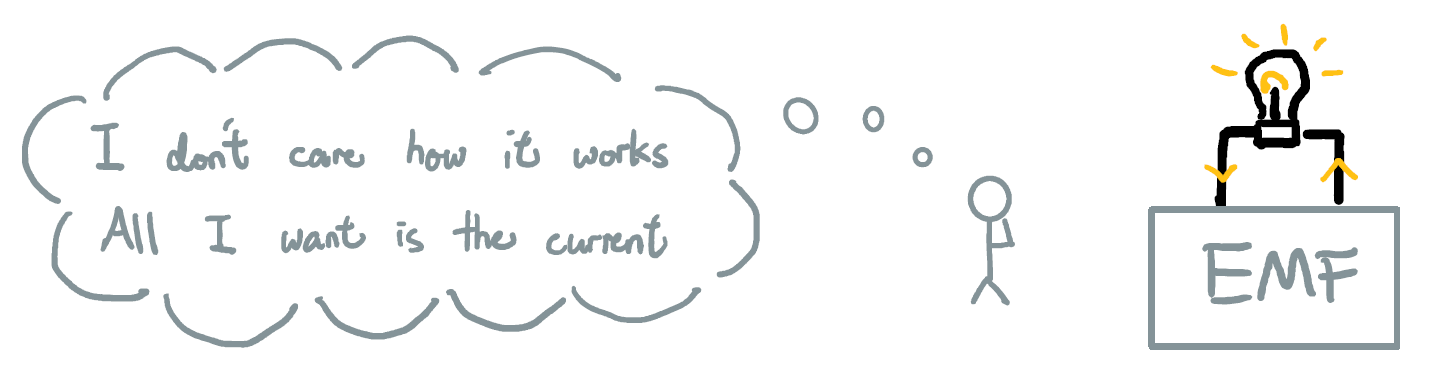
\includegraphics[width=\textwidth]{dun_care}
    \end{minipage}
\end{center}

\vskip 1ex
The discussions of magnetic induction
involves two kinds of EMF:
\begin{itemize}
    \item \bf{\ul{Motional EMF}} 
    \begin{itemize}
        \item Source of energy = Initial motion of the charges.
        \item Can be explained by Lorentz magnetic force.
    \end{itemize}

    \item \bf{\ul{Transformer EMF}}
    \begin{itemize}
        \item Source of energy = Change in magnetic field.
        \item Explanation requires relativity.
    \end{itemize}
\end{itemize}

Historically, they were first discovered as two different phenomena.
Then after a few decades, 
they were unified mathematically as a complete theory of magnetic induction.


\newpage
%%%%%%%%%%%%%%
\subsection{Motional EMF}

Motional EMF was discovered the first time by Faraday, 
with the device which is today known as 
\href{https://en.wikipedia.org/wiki/Homopolar_generator}{Faraday disc} or Faraday wheel.

\begin{center}
    \begin{minipage}{0.28\linewidth}
        \centering
        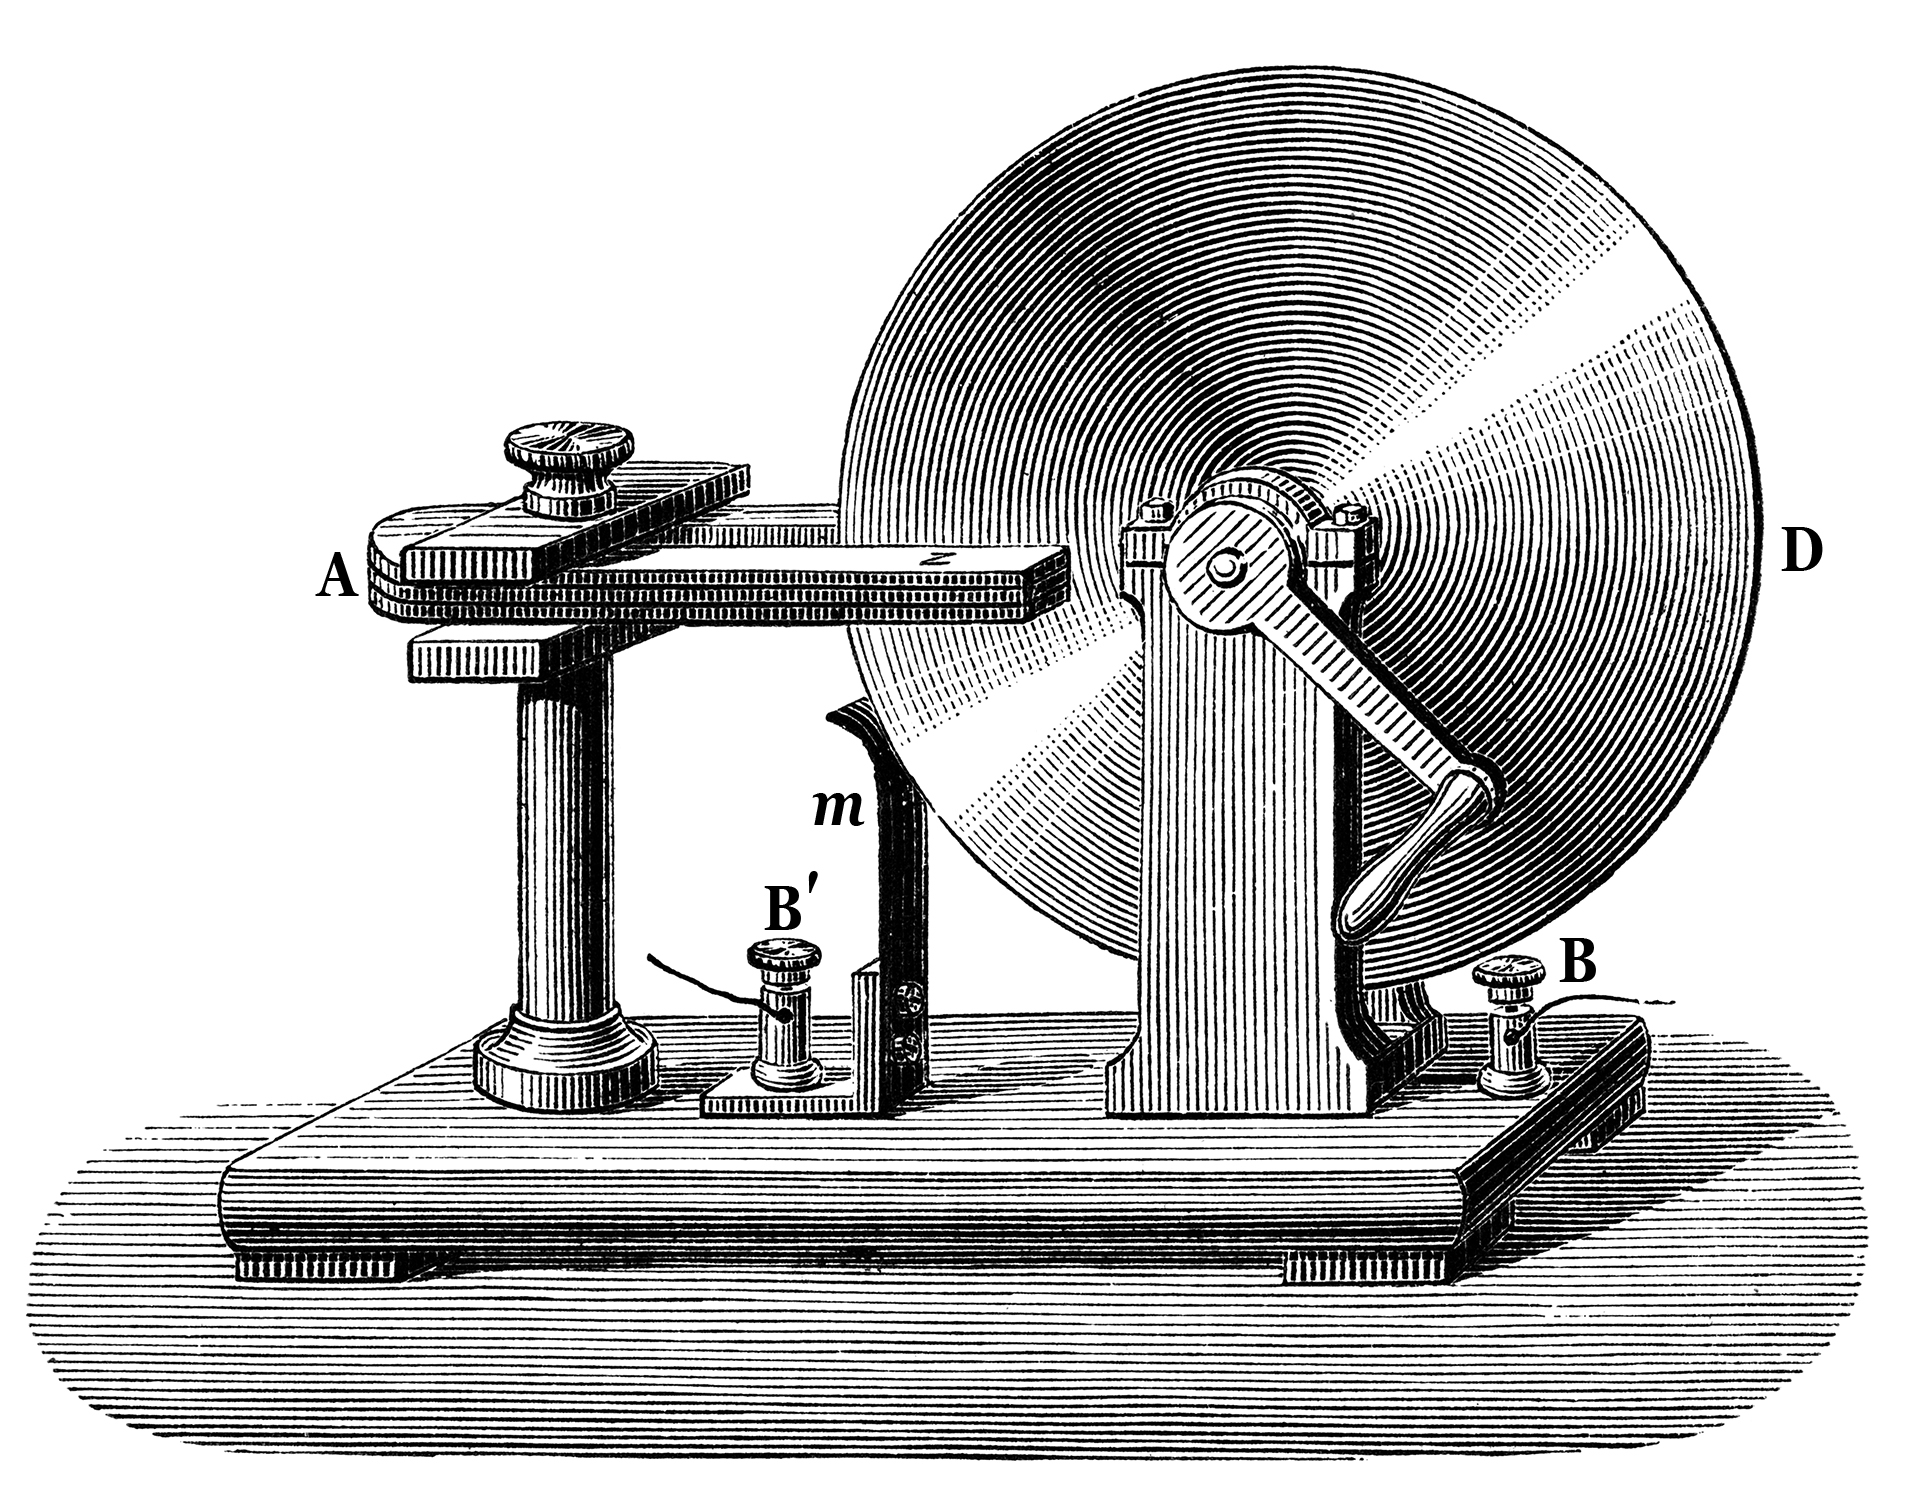
\includegraphics[width=\textwidth]{Faraday_disk_generator}\\
        (Image from \href{https://en.wikipedia.org/wiki/Faraday%27s_law_of_induction#/media/File:Faraday_disk_generator.jpg}{Wiki})
    \end{minipage}
    \hspace{0.02\textwidth}
    \begin{minipage}{0.6\linewidth}
        \begin{itemize}
            \item D = A metal disc
            \item A = A Magnet creating B-field through the disc
            \item Current can conduct through B $\rightarrow$ Disc $\rightarrow$ m $\rightarrow$ B'
        \end{itemize}

        When the disc turns, EMF is observed between B and B'.
    \end{minipage}
\end{center}

\vskip 2ex
To understand how motional EMF is created,
we can first think of what happens if charges are subject to a second kind of force
in addition to the electric forces between each other.
\begin{itemize}
    \item If there is only electric force,
    charges freely distribute themselves until net electric force is $0$.
    i.e. Electric potential is the same everywhere.
    \begin{center}
        \begin{minipage}{0.3\linewidth}
            \centering
            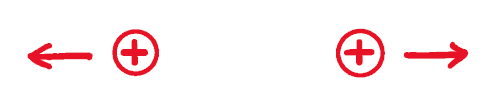
\includegraphics[width=0.8\textwidth]{extraF1}\\
            Only Electric force present
        \end{minipage}
        {\huge \quad$\Rightarrow$\quad}
        \begin{minipage}{0.35\linewidth}
            \centering
            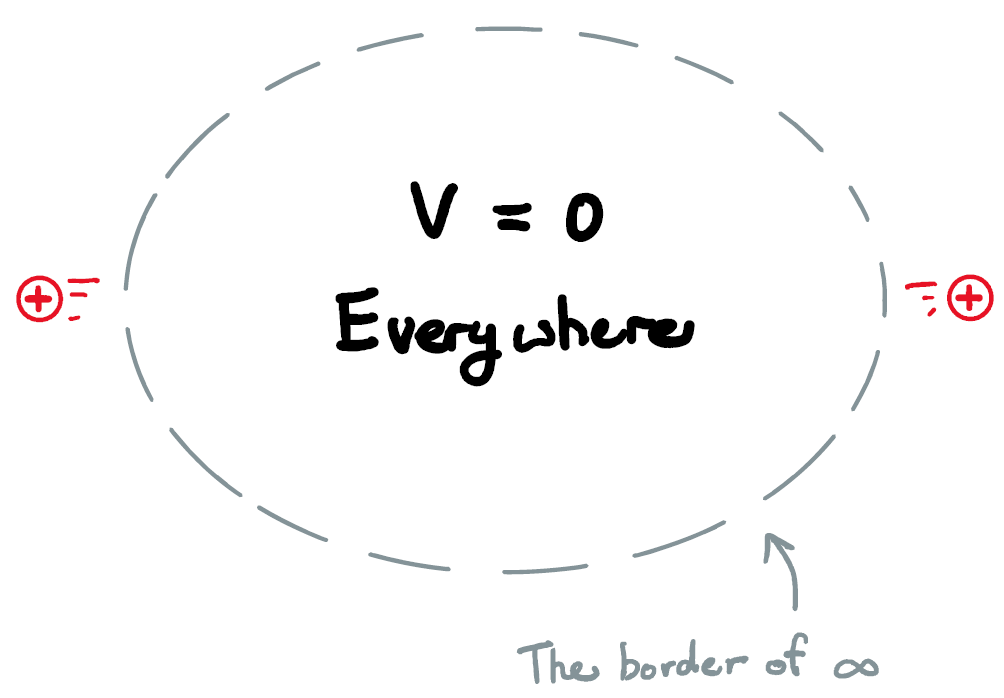
\includegraphics[width=\textwidth]{extraF2}
        \end{minipage}
    \end{center}

    \item With a second kind of force in the space, 
    charges distribute themselves to new equilibrium positions -  
    making electric potential no longer a constant of position.
    i.e. Creating electric potential difference.
    \begin{center}
        \begin{minipage}{0.3\linewidth}
            \centering
            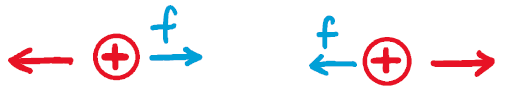
\includegraphics[width=0.8\textwidth]{extraF3}\\
            E.g. Adding static friction in the space
        \end{minipage}
        {\huge \quad$\Rightarrow$\quad}
        \begin{minipage}{0.3\linewidth}
            \centering
            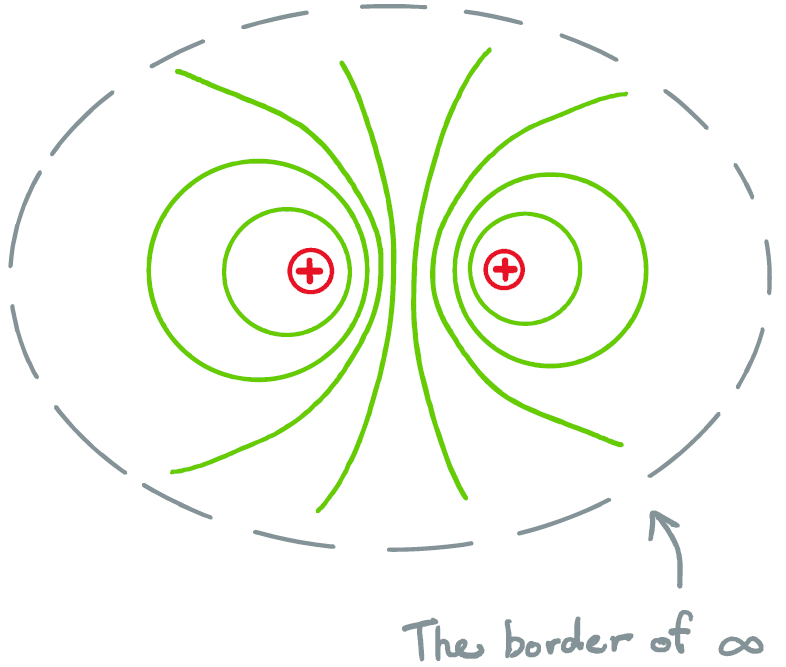
\includegraphics[width=\textwidth]{extraF4}
        \end{minipage}
    \end{center}

\end{itemize}


The situation becomes weird \bf{if the second force is the Lorentz magnetic force},
whose magnitude is proportional to the charges' velocities.
\bf{The potential difference can be maintained only if the charges are moving}.



%%%%%%%%%%%%%%
\subsubsection{The Moving Rod Model}

\iffalse
Suppose there are some charges in an infinitely long conducting rod.
When the charge is given some initial velocity perpendicular to the rod
(e.g. we give the rod a push),
the charge will start to move in a circlar trajectory, 
and the rod will be dragged along by the charge. \\

(If the rod is restricted to move horizonally, it becomes SHM.)

\insertFig{pipe SHM, make the rod infinitely long!}

\fi

{\scriptsize (This is probably the most common model for studying motional EMF for the first time.)}\\

Consider a finite long conducting rod that contains some charges. 
We give the rod a small horizontal push initially.
\begin{enumerate}
    \item The charges cannot escape from the rod - 
    they must move at the same horizontal velocity as the rod.

    \item According to the direction of Lorentz force, 
    the charges will receive accelerations in the direction along the rod.

    \item However because the rod is closed off at its ends, 
    charges near the ends will be pushed against the end walls and cannot move.
    Very soon, charge will accumulate.

    \item The accumulated charges build up a E-field (i.e. potential difference) between the ends of the rod. 
    All charges stop moving vertically when the force from the built-up E-field balance the magnetic force, 
    i.e. when $q\norm{E} = q\norm{v}\norm{B}$.
\end{enumerate}

\begin{center}
    \begin{minipage}{0.2\linewidth}
        \centering
        \blue{Cannot go}\\\blue{beyond the wall}\\
        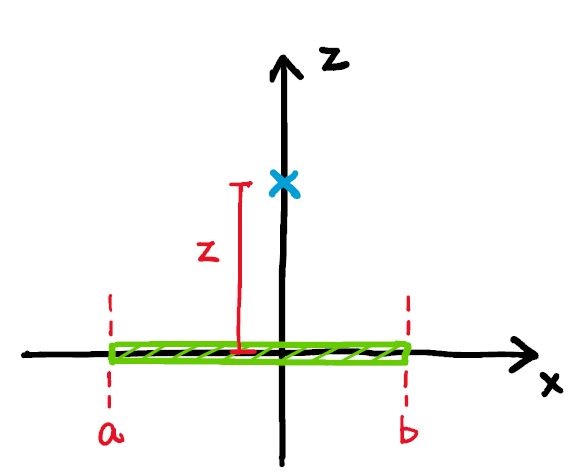
\includegraphics[width=0.93\textwidth]{rod1}\\[-1ex]
        \red{Cannot go}\\\red{beyond the wall}\\
    \end{minipage}
    {\huge \quad$\Rightarrow$\quad}
    \begin{minipage}{0.2\linewidth}
        \centering
        \blue{Accumulating -ve charges}\\
        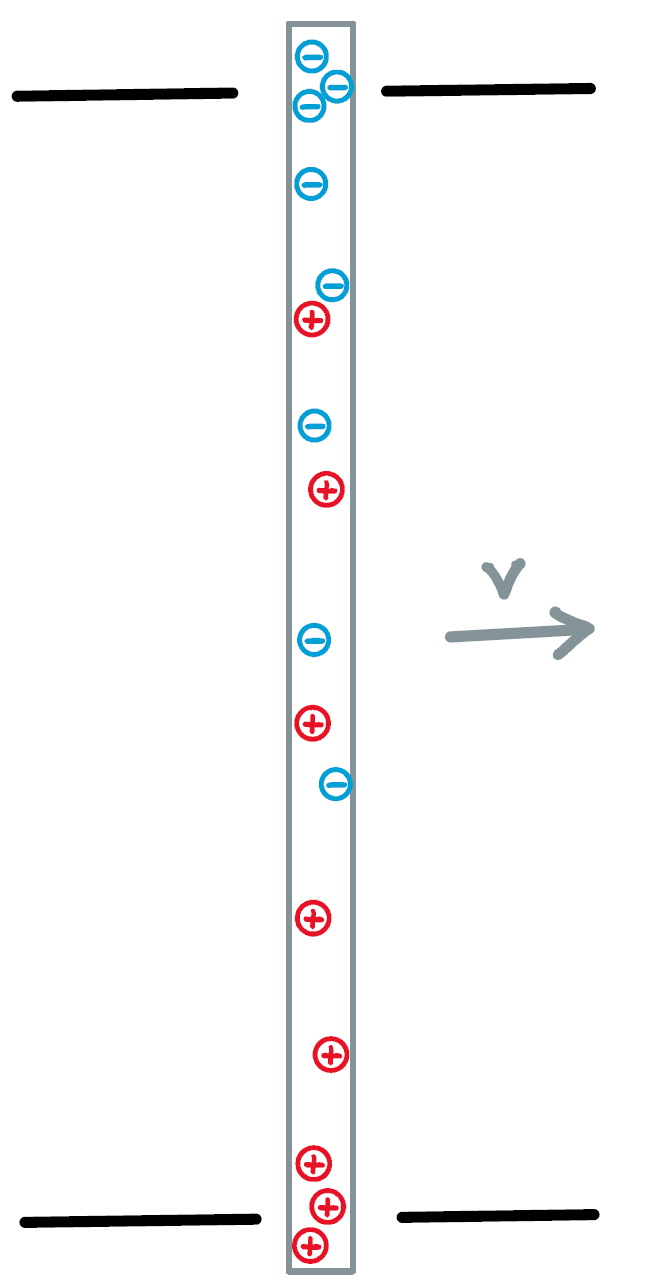
\includegraphics[width=\textwidth]{rod2}\\
        \red{Accumulating +ve charges}
    \end{minipage}
    {\huge \quad$\Rightarrow$\quad}
    \begin{minipage}{0.2\linewidth}
        \centering
        \green{Creating}\\\green{potential difference}\\
        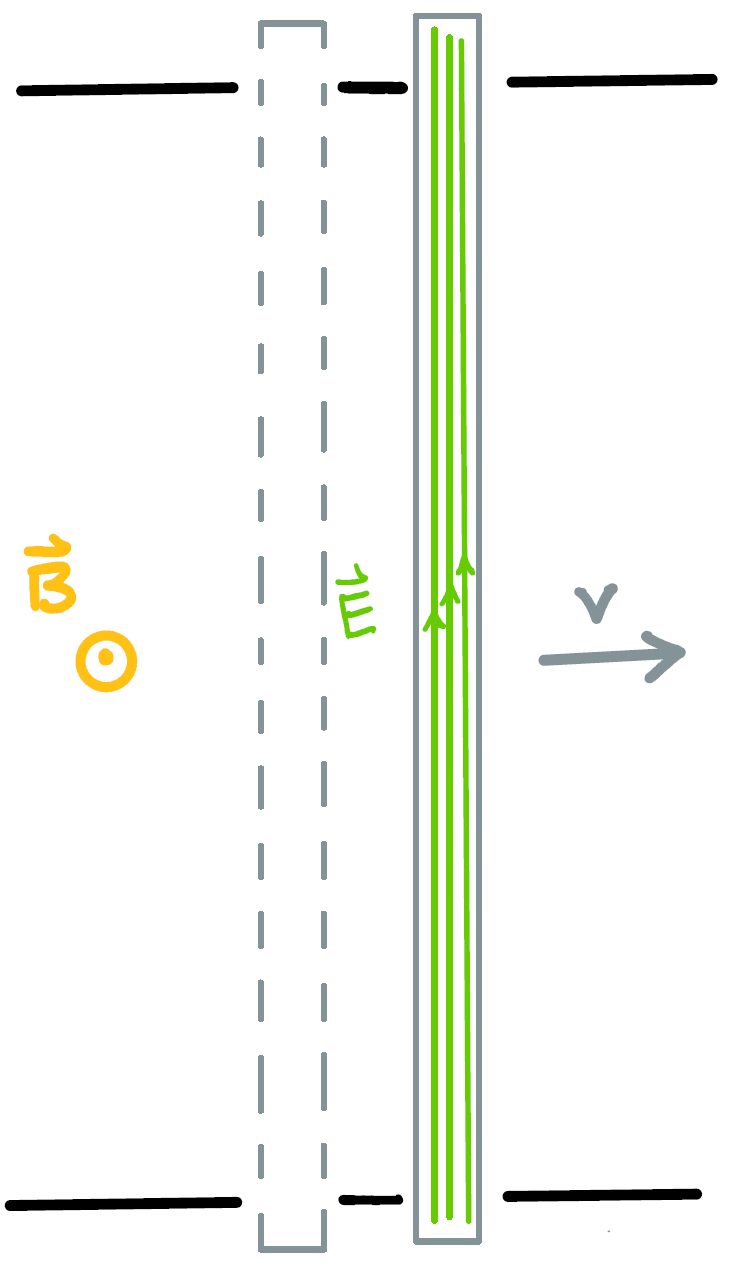
\includegraphics[width=\textwidth]{rod3}\\
        \phantom{AAA}\\\phantom{AAA}
    \end{minipage}
\end{center}

\vskip 1em
Note that such "equilibrium" is only along the vertical direction. 
The rod and charges must maintain some horizontal motion to keep the magnetic force "alive".
If the rod suddenly stop moving,  
the built-up potential difference, and thus the stored energy, will be released.
\begin{center}
    \bf{The rod can be used to drive current. \\
    It is a EMF source - but only when it is moving!}
\end{center}

\begin{center}
    \begin{minipage}{0.3\linewidth}
        \centering
        If the EMF source comes from electrochemistry,\\
        it is called a \cul[red]{battery}.
    \end{minipage}\quad
    \begin{minipage}{0.1\linewidth}
        \centering
        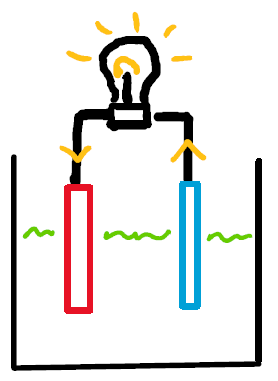
\includegraphics[height=7em]{emf_battery}
    \end{minipage}
    \qquad\vline\qquad
    \begin{minipage}{0.1\linewidth}
        \centering
        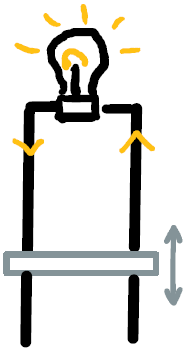
\includegraphics[height=7em]{emf_generator}
    \end{minipage}
    \quad
    \begin{minipage}{0.3\linewidth}
        \centering
        If the EMF source comes from moving conductor,\\
        it is called a \cul[red]{generator}.
    \end{minipage}
\end{center}


%%%%%%%%%%%%%%
\subsubsection{Energy Conservation in Moving Wire}

An alternative explanation of motional EMF is that,
it is a result of energy conservation given that the only W.D. comes from Lorentz magnetic force.\\

Let the B-field be constant and in $\hhat{z}$ direction, i.e. $\vvec{B}=B_z\hhat{z}$.
When the charge on its mid-way to its new equilibrium position, 
\begin{itemize}
    \item The charge's velocity is non-zero in both directions - 
    $+\hhat{y}$ motion from the rod's initial motion,
    and $+\hhat{x}$ motion from acceleration by Lorentz force.

    \item Lorentz force is then in the direction of $\vvec{v}\cross\vvec{B}$,
    composed of a $+\hhat{x}$ and a $-\hhat{y}$ component.
    
\end{itemize} 

\begin{center}
    \begin{minipage}{0.2\linewidth}
        \centering
        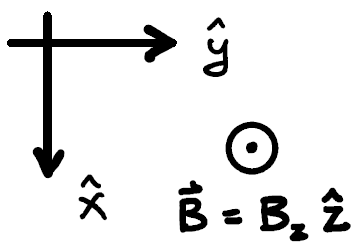
\includegraphics[height=3em]{energy0}\\[1em]
        $\qty(\substack{\text{x-y direction here}\\\text{is roatated by}\\\text{90 degree}})$
    \end{minipage}
    \ 
    \begin{minipage}{0.3\linewidth}
        \centering
        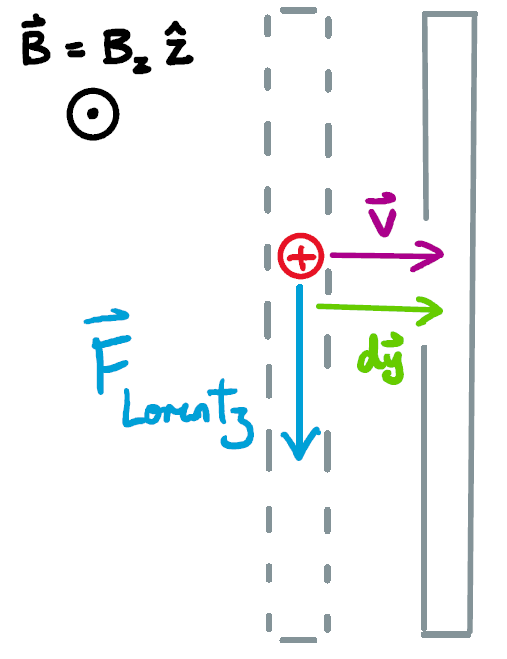
\includegraphics[height=12em]{energy1}
    \end{minipage}
    {\huge\ $\Rightarrow$\ }
    \begin{minipage}{0.3\linewidth}
        \centering
        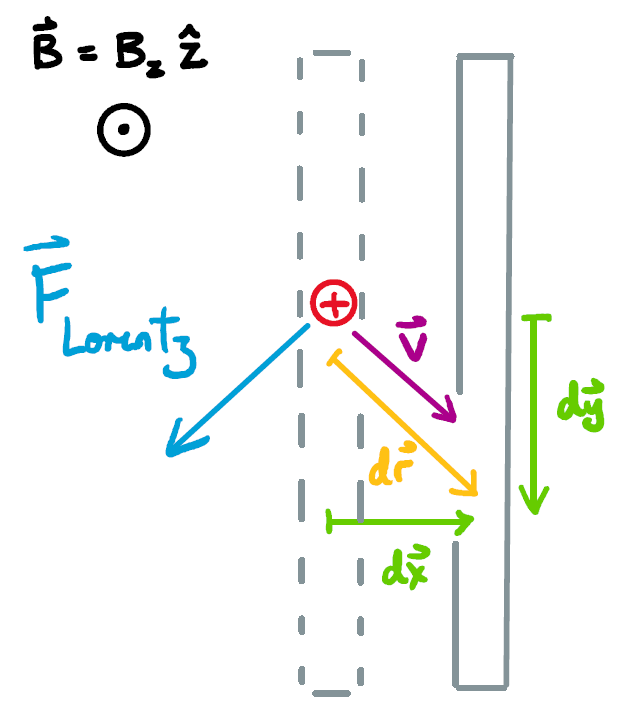
\includegraphics[height=12em]{energy2}
    \end{minipage}
\end{center}

\bf{Although Lorentz force is accelerating the charge's $x$ motion,
at the same time it is decelerating the charge's $y$ motion.}
%And because the charge must stay inside the rod,
%the rod will also be slowed down.
%So \bf{this is a process of conservation of energy - 
%from the horizontal KE of the rod to the vertical KE of charge inside the rod}.\\
We can show that energy is conserved under this change in the charge's motion 
by looking at the W.D. under a small displacement $\dd{\vvec{r}}$.

\begin{enumerate}

    \item Always remember: Work done on a charge by magnetic force is always $0$, 
    because $\vvec{F}_B$ is perpendicular to the travelling direction $\dd{\vvec{r}}$,
    (i.e. same direction as $\vvec{v} =\dv{\vvec{r}}{t}$).
    \aleq{
        \text{W.D.} &= \vvec{F}_B \cdot \dd{\vvec{r}} = q(\vvec{v}\cross\vvec{B})\cdot\dd{\vvec{r}} = 0
    }
    
    \item Meanwhile we can separate this W.D. into contributions along $x$ and $y$ direction:
    \aleq{
        \text{W.D.} &= q\qty[(\vvec{v}_x+\vvec{v}_y)\cross \vvec{B}]\cdot \qty(\dd{\vvec{x}}+\dd{\vvec{y}})\\
        %
        &= \cus[blue]{\ccancelto[blue]{0}{q(\vvec{v}_x\cross\vvec{B})\cdot\dd{\vvec{x}}}}
            {\substack{\vvec{v}_x\cross \vvec{B}= v_xB_z(\hhat{x}\cross \hhat{z})
                \\\phantom{\vvec{v}_{xi} \vvec{B}}=v_xB_z(-\hhat{y})\\[0.5ex]
                \text{Dotting with }\hhat{x}\text{ gives }0}}
            %
            + q(\vvec{v}_x\cross\vvec{B})\cdot\dd{\vvec{y}} 
            + q(\vvec{v}_y\cross\vvec{B})\cdot\dd{\vvec{x}}
            %
            + \cus[blue]{\ccancelto[blue]{0}{q(\vvec{v}_y\cross\vvec{B})\cdot\dd{\vvec{y}}}}
            {\substack{\vvec{v}_y\cross \vvec{B}= v_yB_z(\hhat{y}\cross \hhat{z})
                \\\phantom{\vvec{v}_{xi} \vvec{B}}=v_yB_z(\hhat{x})\\[0.5ex]
                \text{Dotting with }\hhat{y}\text{ gives }0}}\\[1ex]
        %
        &= (-qv_xB_z\hhat{y})\cdot \dd{\vvec{y}} + (qv_yB_z\hhat{x}) \cdot \dd{\vvec{x}}\\[1ex]
        %
        &= \cus[red]{(-qv_xB_z)\dd{y}}
                {\substack{\text{W.D. on charge}\\\text{in }\hhat{y}\text{ direction}\\[0.5ex]\sim\ F_y \dd{y}}}
            \ +\ \cus[red]{(qv_yB_z)\dd{x}}
                {\substack{\text{W.D. on charge}\\\text{in }\hhat{x}\text{ direction}\\[0.5ex]\sim\ F_x \dd{x}}}\\[1ex]
        %
        &\equiv 0 \quad\text{\scriptsize (Required by magnetic force)}
    }

    To always hold true, these two W.D. must have equal magnitude but opposite sign.

    \item When charges accumulate at the ends of the rod,
    equilibrium happens when $q\vvec{E} = q\vvec{v}\cross\vvec{B}$.
    So when a charge climbs up the E-field for a small distance $\dd{\vvec{x}}$,
    it will gain a PE of:
    \addArrow[blue]{d_emf}{(0,-2ex)}{\scriptsize The potential gain\\[-1ex]\scriptsize i.e. EMF}{(0,-0.7ex)}{(2ex,-1ex)}
    \aleq{
        q\dd{\tkn{d_emf}{\cul[blue]{\epsilon}}} 
            \ \equiv\ (q\vvec{E})\cdot\dd{\hhat{x}}
            = q(\vvec{v}\cross\vvec{B})\cdot\dd{\hhat{x}}
            = (qv_yB_z)\dd{x}
    }
    
    \vskip 1.5em

\end{enumerate}

We can see that these 3 terms are equal:
\aleq{
    \cus[blue]{q\dd{\epsilon}}
    {\substack{\text{Built-up}\\\text{electric PE}}}
    %
    \quad = \quad
    %
    \cus[red]{(qv_yB_z)\dd{x}}
    {\substack{\text{W.D. on charge}\\\text{in }\hhat{x}\text{ direction}}}
    %
    \quad = \quad
    %
    \cus[red]{(qv_xB_z)\dd{y}}
    {\substack{\text{W.D. on charge}\\\text{in }\hhat{y}\text{ direction}}}
}

which implies an energy conservation process:

\begin{itemize}
    \item To build up the potential in the rod, 
    We must do work to the charges along the rod ($x$ direction) to drive the charge against the built-up potential.
    
    \item Lorentz magnetic force supplies this energy to do work to the charges along the rod, 
    by doing work against the charge's motion in the $y$ direction.
    
\end{itemize} 

\vskip 1ex
%%%%%%%%%%%%%%
\subsubsection{Magnetic Flux - A Geometrical Relation}

The idea of magnetic flux comes from generalizing motional EMF by vector calculus.
To begin with, transform the rod into a wire with arbituary shape which moves in an arbituary fashion.

\begin{center}
    \begin{minipage}{0.3\linewidth}
        \centering
        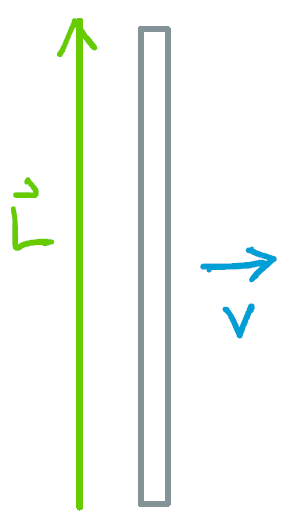
\includegraphics[height=7em]{seg1}
    \end{minipage}
    {\huge \ $\Rightarrow$\ }
    \begin{minipage}{0.3\linewidth}
        \centering
        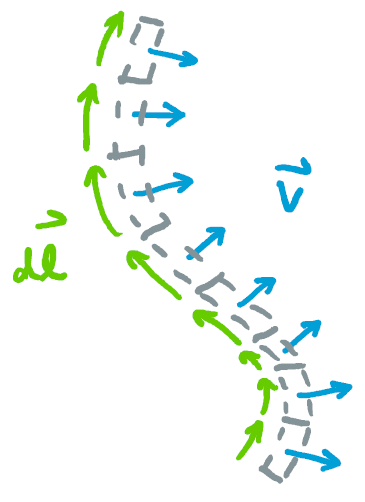
\includegraphics[height=7em]{seg2}
    \end{minipage}
\end{center}

The total EMF generated can be regarded as the sum of contribution by many infinitestimal segments - 
For the $i$\Nth segment,

\begin{minipage}{0.6\linewidth}
    \begin{itemize}
        \item has a (length) + (orientation) labeled by $\dd{\vvec{l}_i}$.
        \item is moving in velocity $\vvec{v}_i$.
    \end{itemize}
\end{minipage}
\begin{minipage}{0.3\linewidth}
    \centering
    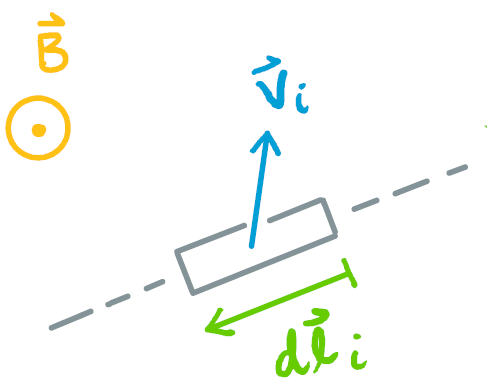
\includegraphics[height=7em]{seg3}
\end{minipage}

\vskip 1.5em
Then with some algebra, the EMF generated in each segment can be written as 
\addArrow[blue]{identity1}{(8ex,0)}
{\scriptsize Vector identity: \\[-1ex]
    \scriptsize $(\vvec{a}\cross\vvec{b})\cdot\vvec{c} = (\vvec{c}\cross\vvec{a})\cdot\vvec{b} = (\vvec{b}\cross\vvec{c})\cdot\vvec{a}$\\[-1ex]
    \scriptsize (i.e. $a\rightarrow b \rightarrow c\rightarrow a$ forming a cycle)}
{(1ex,1ex)}{(11.5ex,2ex)}
\addArrow[red]{identity2}{(6ex,0)}{\scriptsize $\vvec{a}\cross \vvec{b} = -\vvec{b}\cross\vvec{a}$}
{(1ex,1ex)}{(5ex,0.3ex)}
\aleq{
    \dd{\epsilon_i} &= (\vvec{v}_i\cross\vvec{B})\cdot\dd{\vvec{l}_i}\\[1ex]
    &= (\dd{\vvec{l}_i}\cross\vvec{v}_i)\cdot \vvec{B}\tkm{identity1}\\[1ex]
    &= -(\vvec{v}_i\cross\dd{\vvec{l}_i})\cdot \vvec{B}\tkm{identity2}
}


In a short duration $\dd{t}$,
the displacement of the segment is $\vvec{v}_i\dd{t}$.
So we can approximate the swept area by the segment as a parallelogram:
\aleq{
    \qty(\mstack{\text{Swept}\\\text{Area}})
    &= \qty(\mstack{\text{Area of parallelogram}\\\text{made by } \vvec{v}_i\dd{t} \text{ \& }\dd{\vvec{l}}_i})\\
    &\approx \norm{\vvec{v}_i \dd{t}}\norm{\dd{\vvec{l}_i}}\sin \qty(\mstack{\text{Angle between}\\\vvec{v}_i\dd{t} \text{ \& }\dd{\vvec{l}}_i})\\
    &= (\vvec{v}_i \dd{t})\cross(\dd{\vvec{l}_i})\\
    %
    \dvv{t} \qty(\mstack{\text{Swept}\\\text{Area}}) &= \vvec{v}_i\cross \dd{\vvec{l}}_i
} 

\begin{center}
    \begin{minipage}{0.15\linewidth}
        \centering
        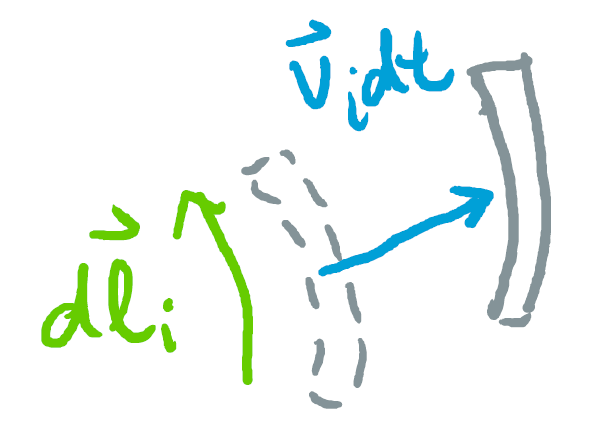
\includegraphics[width=\textwidth]{swept1}
    \end{minipage}
    {\huge \quad $\Rightarrow$\quad }
    \begin{minipage}{0.15\linewidth}
        \centering
        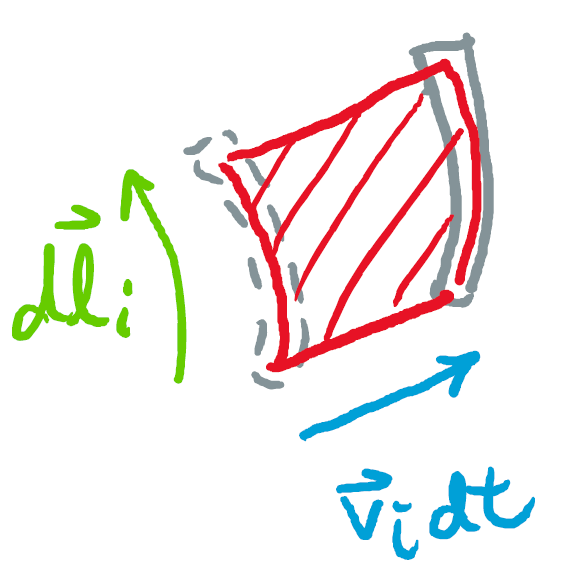
\includegraphics[width=\textwidth]{swept2}
    \end{minipage}
    {\huge \quad $\Rightarrow$\quad }
    \begin{minipage}{0.15\linewidth}
        \centering
        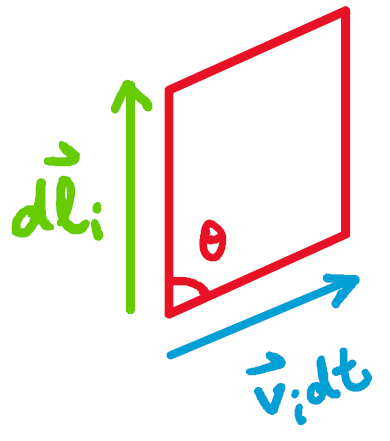
\includegraphics[width=\textwidth]{swept3}
    \end{minipage}
\end{center}

We can now relate EMF generated in the whole wire with swept area by the wire as:
\aleq{
    \sum \epsilon = -\sum_{\substack{\text{All}\\\text{segments}}}
        \qty[(\vvec{v}_i\cross\dd{\vvec{l}_i})\cdot \vvec{B}]
    &= -\sum_{\substack{\text{All}\\\text{segments}}} 
        \qty[\dvv{t}\qty(\mstack{\text{Swept}\\\text{area}})_i\cdot \vvec{B}]\\
    &= -\dvv{t}\sum_{\substack{\text{All}\\\text{segments}}}
        \qty[\qty(\mstack{\text{Swept}\\\text{area}})\cdot \vvec{B}]
} 

When the segments are infinitestimally short, the sum becomes integral.
\aleq{
    \epsilon = -\int (\vvec{v}\cross\dd{\vvec{l}_i})\cdot\vvec{B}
    &= -\dvv{t}\qty[\iint_{\substack{\text{Swept}\\\text{area}}}\vvec{B}\cdot\dd{\vvec{s}}]\\
    &= -\dvv{t}\qty(\mstack{\text{Magnetic flux through}\\\text{the swept area}})
}

Pay attention to the depedendence to $t$ on the RHS:
\begin{itemize}
    \item The B-field $\vvec{B}$ is static. It is not a function of $t$.
    
    \item $\dd{\vvec{s}}$ is just a notation saying that this is a flux integral. 

    \item The only thing that depends on $t$ is the \cul[red]{integration range}.
\end{itemize}

So to be more accurate, the equation of motional EMF should be written as 
\aleq{
    \Aboxed{
        \epsilon_\blue{\text{(motional)}} 
        = \int_{\substack{\text{along a wire}\\\text{of shape of }\cul[red]{\cul[red]{l(t)}}}} 
            (\vvec{v}\cross\vvec{B})\cdot \dd{\vvec{l}}
        = -\dvv{t} \iint_{\substack{\text{Area }\cul[red]{\cul[red]{S(t)}}\\\text{swept by wire}}} 
            \vvec{B}\cdot\dd{\vvec{s}}
    }
}

to emphasize that it is the wire's shape / swept area varying with time.



%%%%%%%%%%%%%%
\subsection{Transformer EMF}

Transformer EMF was also discovered by Faraday,
with a primitive toroidal transformer.
\begin{center}
    \begin{minipage}{0.25\linewidth}
        \centering
        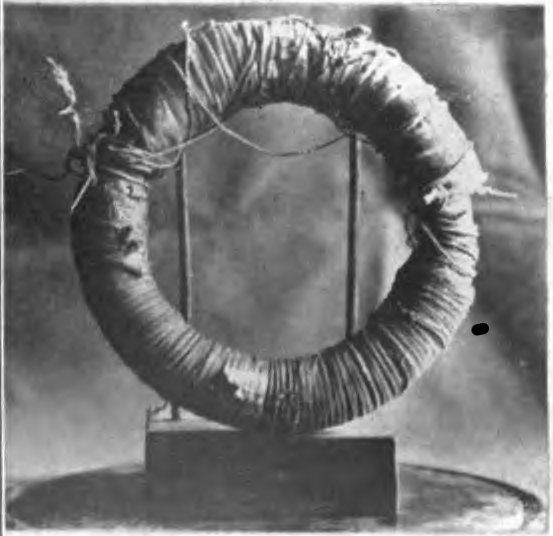
\includegraphics[width=\textwidth]{Faraday_ring_transformer}\\
        (Image from \href{https://commons.wikimedia.org/wiki/File:Faraday_ring_transformer.jpg}{wiki})
    \end{minipage}
    \hspace{0.05\textwidth}
    \begin{minipage}{0.6\linewidth}
        \centering
        When the current on one side is switch on / switch off,
        EMF is observed on the other side of the transformer.\\[1em]
        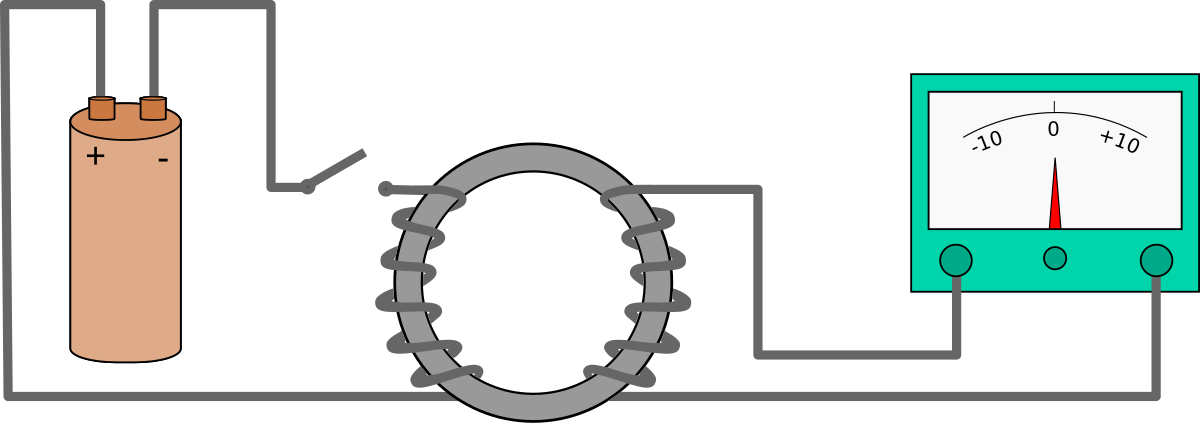
\includegraphics[width=0.6\textwidth]{Faraday_emf_experiment}
    \end{minipage}
\end{center}

\vskip 1em
In modern explanation, 
transformer EMF can only be explained by relativity - 
motional EMF and transformer EMF are the same phenomenon being observed in different reference frame. 

\begin{center}
    \begin{minipage}{0.4\linewidth}
        \centering
        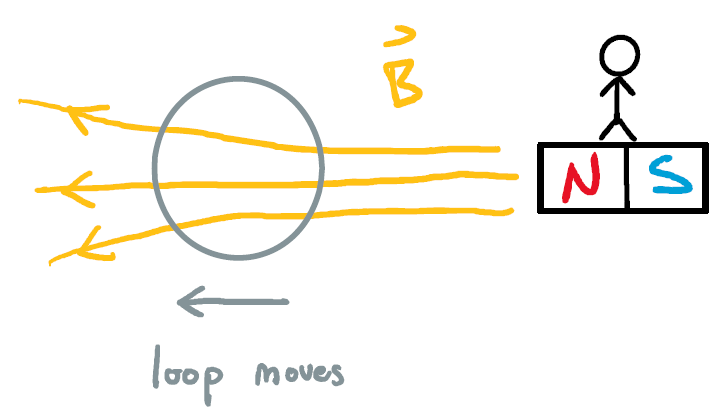
\includegraphics[width=0.7\textwidth]{transformer1}\\
        EMF generated due to\\ motion of the ring
    \end{minipage}
    {\huge \quad $\Leftrightarrow$\quad }
    \begin{minipage}{0.4\linewidth}
        \centering
        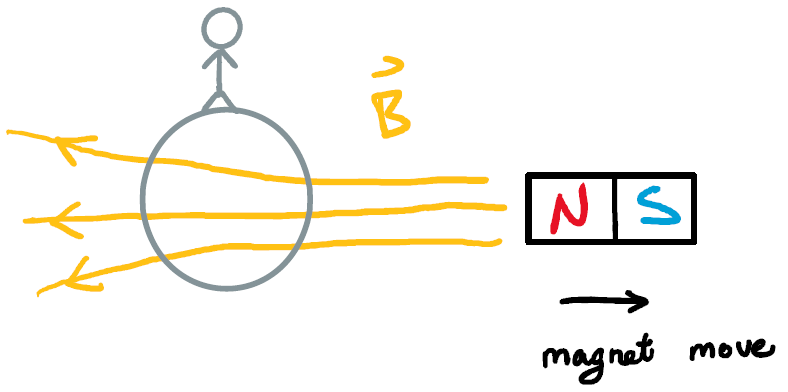
\includegraphics[width=0.75\textwidth]{transformer2}\\
        EMF generated due to changing magnetic field strength
    \end{minipage}
\end{center}

\vskip 1ex
%%%%%%%%%%%%%%
\subsubsection{Induced E-field}

Imagine that we are in a reference frame which we only observe transformer EMF,
i.e. the charge is stationary while B-field is the only thing changing with time.
\begin{itemize}
    \item The direct interaction between the charge and B-field 
    - Lorentz magnetic force must be $0$.
    \item But we somehow observe the charge moving (due to some potential difference).
\end{itemize}

This implies there is a second way how B-field can interact with charges.
To complete the theory, an induced E-field is proposed.

\begin{center}
    \begin{minipage}{0.4\linewidth}
        \centering
        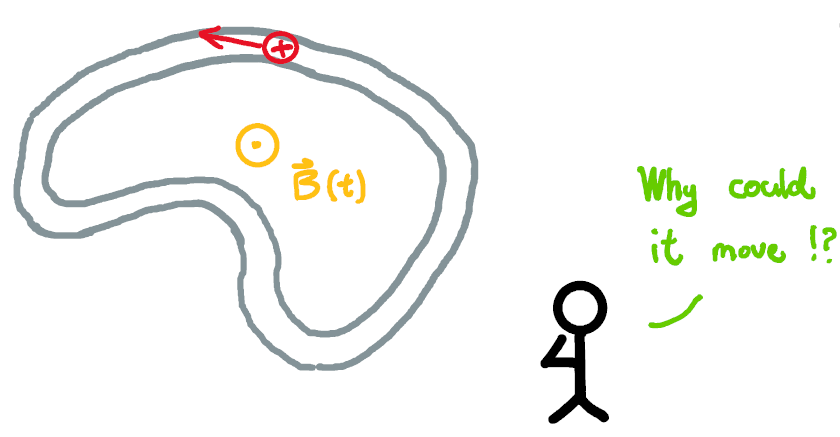
\includegraphics[width=0.85\textwidth]{induce1}\\
        Observation:\\ Charge moves without force
    \end{minipage}
    {\huge \quad $\Rightarrow$\quad }
    \begin{minipage}{0.4\linewidth}
        \centering
        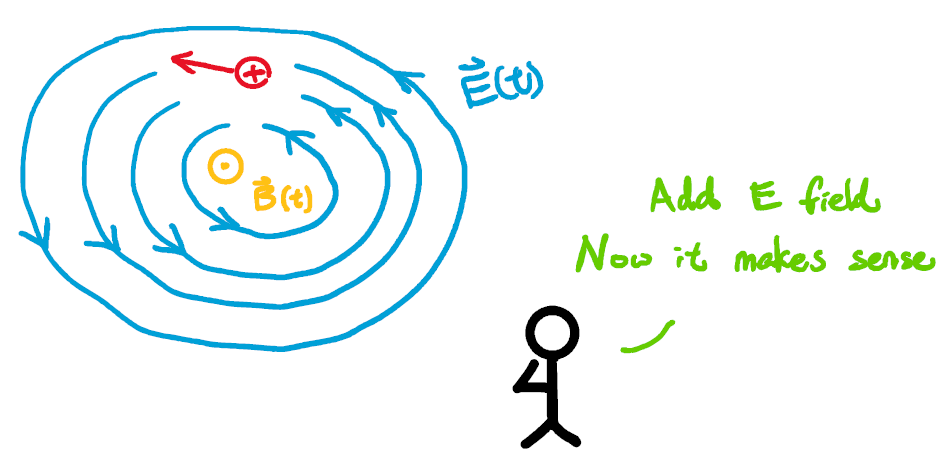
\includegraphics[width=0.9\textwidth]{induce2}\\
        Add induced E-field\\ to fix Newton's \nth{2} law
    \end{minipage}
\end{center}

\newpage
As an analogy, 
the addition of induced E-field is very similar to the reason of 
adding frictious force to accelerating frame.
\begin{center}
    \begin{minipage}{0.4\linewidth}
        \centering
        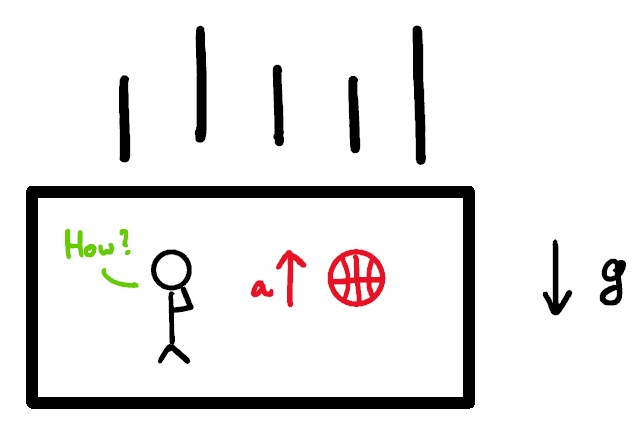
\includegraphics[width=0.6\textwidth]{newton1}\\
        Observation:\\ Ball rises up without force
    \end{minipage}
    {\huge \ \ $\Rightarrow$\ \ }
    \begin{minipage}{0.4\linewidth}
        \centering
        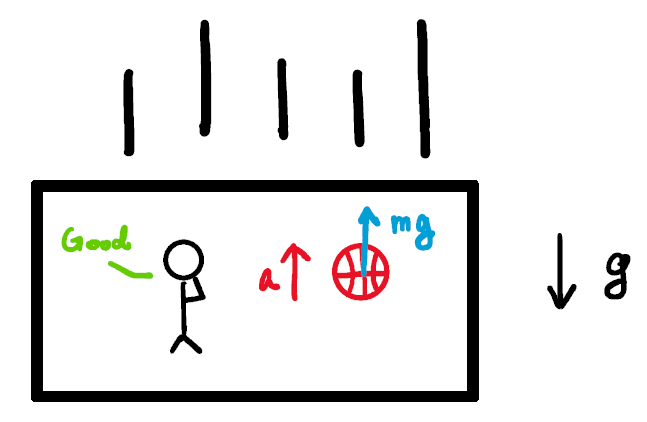
\includegraphics[width=0.6\textwidth]{newton2}\\
        Add ficticious force\\ to fix Newton's \nth{2} law
    \end{minipage}
\end{center}

\vskip 1em
It is experimentally possible to determine the distribution of this E-field.
For example, we can sample the induced EMF using different conductor loops:
\begin{center}
    \begin{minipage}{0.37\linewidth}
        \centering
        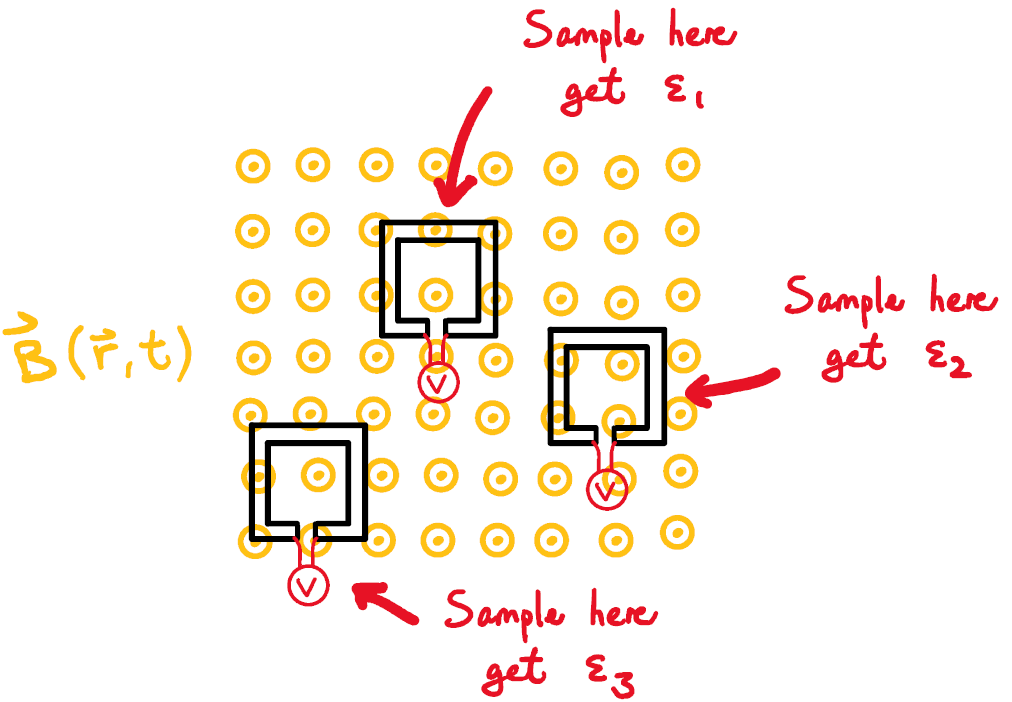
\includegraphics[width=\textwidth]{sample1}
    \end{minipage}
    {\qquad $\xRightarrow{\text{Sampling many loops}}$\ }
    \begin{minipage}{0.37\linewidth}
        \centering
        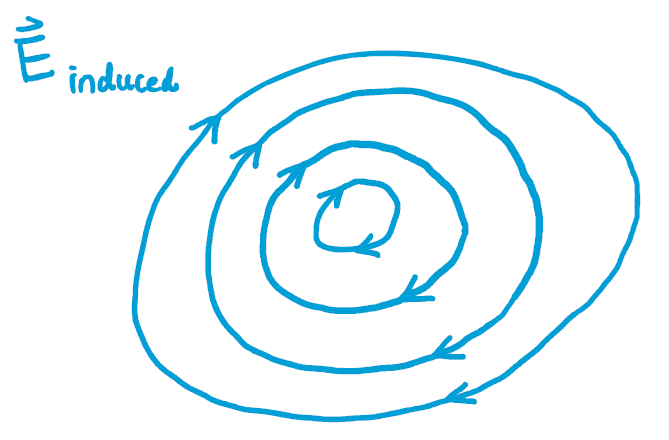
\includegraphics[width=0.75\textwidth]{sample2}
    \end{minipage}
\end{center}

\vskip 1ex
With direct measurements, it was found that
\begin{itemize}
    \item The induced E-field must be in form of loops, 
    i.e. non-conservative.
    Otherwise charges will not run indefinitely in the conductor loops,
    and so cannot be used to drive current.

    \item The induced EMF is proportional to the rate of change of B-field 
    and area of the loop. i.e. 
    \aleq{
        \text{EMF} \ \propto\  \qty(\dvv{t}\vvec{B}(t))\cdot \qty(\mstack{\text{Loop's}\\\text{area}})
    }
\end{itemize}

These observations suggest a mathematical relation in vector calculus:
\aleq{
    \Aboxed{
        \epsilon_\blue{(\text{transformer})} 
        = \oint_{\substack{\text{The}\\\text{loop}}} \vvec{E}_\text{induced}\cdot \dd{\vvec{l}}
        = -\iint_{\substack{\text{The loop's}\\\text{area}}} \qty(\pdvv{\vvec{B}}{t})\cdot \dd{\vvec{s}}
    }
}

The minus sign in front of the surface integral is added to match the sign in motional EMF.



%%%%%%%%%%%%%%
\subsubsection{Maxwell-Faraday Equation}

We have now learnt two ways of creating E-field:
1. emitted by charge or 2. induced by changing B-field. 
In theory, any E-field distribution must be a combination of these two sources.
\aleq{
    \vvec{E}_\text{total} = \vvec{E}_\text{charge} + \vvec{E}_\text{induced}
}

Moreover, recall that E-field created by charges is always conservative.
i.e.
\aleq{
    \oint_{\substack{\text{Any}\\\text{loop}}} \vvec{E}_\text{charge} \cdot\dd{\vvec{l}} = 0
}

So we can add this term into the formula of transformer EMF 
and get the integral form of \bf{Maxwell-Faraday's equation},
the \nth{3} equation from the set of Maxwell's equation:
\aleq{
    \oint_{\substack{\text{The}\\\text{loop}}} \vvec{E}_\blue{\text{induced}} + \vvec{E}_\blue{\text{charge}}\cdot \dd{\vvec{l}}
    = \oint_{\substack{\text{The}\\\text{loop}}} \vvec{E}_\red{\text{total}}\cdot \dd{\vvec{l}}
    = -\iint_{\substack{\text{The loop's}\\\text{area}}} \qty(\pdvv{\vvec{B}}{t})\cdot \dd{\vvec{s}}
}

or simply
\aleq{
    \Aboxed{
        \oint \vvec{E}\cdot\dd{\vvec{l}} = -\iint \qty(\pdvv{\vvec{B}}{t})\cdot\dd{\vvec{s}}
    }
}

With Stoke's theorem,
it can be converted into its differential form:\\
\addAboveArrow[red]{curlEa}{curlEb}{Stokes' Theorem}{2ex}{(0,0.5ex)}
\aleq{
    \tkn{curlEa}{\oint \vvec{E}\cdot\dd{\vvec{l}}} 
    = \iint \tkn{curlEb}{(\curl \vvec{E})} \cdot \dd{\vvec{s}} 
    &= -\iint \qty(\pdvv{\vvec{B}}{t})\cdot\dd{\vvec{s}}\\
    %
    \Aboxed{
        \curl \vvec{E} &= -\pdvv{\vvec{B}}{t}
    }
}


\vskip 1em
%%%%%%%%%%%%%%
\subsection{Summary: Magnetic Flux \& Faraday's Law}

After such lengthy discussion, here again lists the formula of the two EMF:
\begin{itemize}
    \item \bf{\ul{Motional EMF}}: Wire moving, constant B-field
    \aleq{
        \epsilon_\blue{\text{(motional)}} 
        = \int_{\substack{\text{along a wire}\\\text{of shape of }l(t)}} 
            (\vvec{v}\cross\vvec{B})\cdot \dd{\vvec{l}}
        = -\dvv{t} \iint_{\substack{\text{Area }S(t)\\\text{swept by wire}}} 
            \vvec{B}\cdot\dd{\vvec{s}}
    }
    
    \item \bf{\ul{Transformer EMF}}: Stationary loop , changing B-field
    \aleq{
        \epsilon_\blue{(\text{transformer})} 
        = \oint_{\substack{\text{The}\\\text{loop}}} \tkn{E_tot}{\vvec{E}} \cdot \dd{\vvec{l}}
        = -\iint_{\substack{\text{The loop's}\\\text{area}}} \qty(\pdvv{t}\vvec{B}(t))\cdot \dd{\vvec{s}}
    }
    \addArrow[green]{E_tot}{(0,-4ex)}
    {\scriptsize No longer need to distinguish\\[-1ex]\scriptsize induced E or total E}
    {(0,-1ex)}{(5ex,-1ex)}
\end{itemize}

\vskip 3ex
We can see a similiarity - 
both of the EMF can be expressed as a combination of time derivative and flux integral of B-field.
If we close the wire in motional EMF to form a loop, let it sweep some area, 
and at the same time vary the B-field, 
we will observe the EMF contributed from both effects.

\begin{center}
    \begin{minipage}{0.4\linewidth}
        \centering
        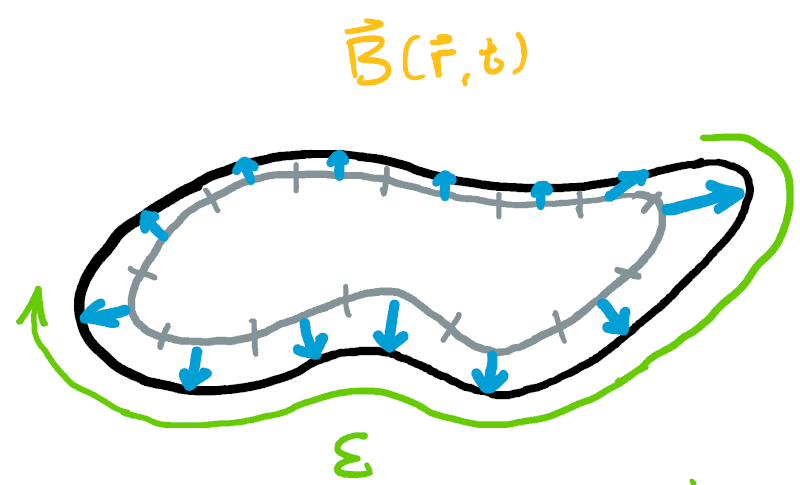
\includegraphics[width=0.7\textwidth]{loop1}\\
        When the loop changes its shape and B-field changes happen together\\
        \phantom{A}
    \end{minipage}
    {\huge \ \ $\Rightarrow$\ \ }
    \begin{minipage}{0.4\linewidth}
        \centering
        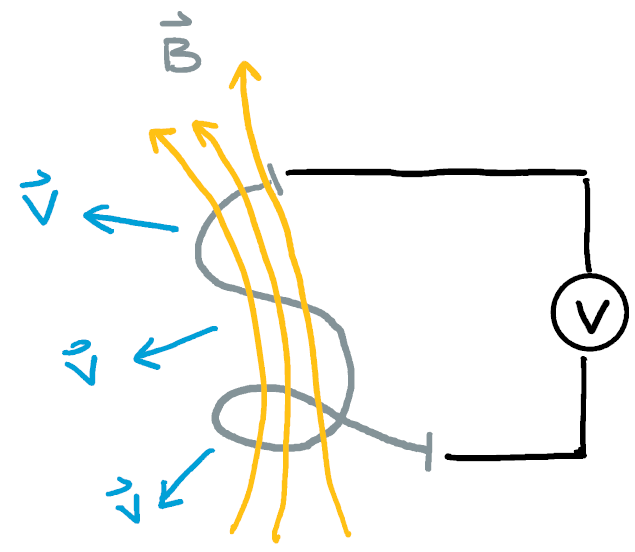
\includegraphics[width=0.6\textwidth]{loop2}\\
        The effective EMF is the rate of change of the magnetic flux\\ in the red area
    \end{minipage}
\end{center}

While mathematically, the two EMF can be merged like product rule of differentiation.
\addBelowArrow[red]{d11}{d12}{\scriptsize $\dv{t}$ only to\\[-0.8ex] \scriptsize integration range}{-3ex}{(0,-1ex)}
\addArrow[green]{b1}{(0,-4ex)}{\scriptsize B-field\\[-1ex] \scriptsize keep constant}{(0,-1ex)}{(1ex,-1ex)}
\addBelowArrow[red]{d21}{d22}{\scriptsize $\dv{t}$ only to\\[-0.8ex] \scriptsize B-field}{-2ex}{(0,-1ex)}
\addArrow[green]{b2}{(0,-3ex)}{\scriptsize integration range\\[-1ex] \scriptsize keep constant}{(0,-1ex)}{(-3ex,-1ex)}
\aleq{
    \epsilon_\blue{\text{(motional)}} + \epsilon_\blue{(\text{transformer})}
    %
    &= -\qty( \tkn{d11}{\dvv{t}} \iint_{\substack{\text{Area }S(t)\\\tkn{d12}{\text{swept by loop}}}} 
        \tkn{b1}{\vvec{B}}\cdot\dd{\vvec{s}}
    %
    \quad+\quad
    %
    \iint_{\substack{\text{The loop's}\\\tkn{b2}{\text{area}}}} 
        \qty(\tkn{d21}{\pdvv{t}}\tkn{d22}{\vvec{B}(t)})\cdot \dd{\vvec{s}})\\[4em]
    %
    &= -\dvv{t}\cub[yellow]{\qty(\iint_{\substack{\text{Area }S(t)\\\text{swept by loop}}} \vvec{B}(t)\cdot\dd{\vvec{s}})}
    {\text{Total magnetic flux through the loop}}
    \qquad\qquad
    \gray{\qty(\substack{\text{Just like }\dd{(uv)} = u\dd{v} + v\dd{u}\\\text{But no rigorous proof here}})}
    %
    %\epsilon_\text{total} &= \dvv{t}\qty(\mstack{\text{Magnetic}\\\text{flux}})
}

\vskip 1ex
This is exactly the description of \bf{Faraday's law of induction}:
\aleq{
    \Aboxed{
        \mstack{\text{Any induced EMF}\\[0.5ex]\text{appear}} 
        \qquad\Leftrightarrow\qquad 
        \mstack{\text{There are time-varying}\\[0.5ex]\text{magnetic flux}}
    }
}

\vskip 1em
In addition, the line integral part shows the origin of the EMF's energy:
\aleq{
    \epsilon_\blue{\text{(motional)}} + \epsilon_\blue{(\text{transformer})}
    %
    &= \oint_{\substack{\text{along a loop}\\\text{of shape of }l(t)}} 
            (\vvec{v}\cross\vvec{B})\cdot \dd{\vvec{l}}
        + \oint_{\substack{\text{The}\\\text{loop}}} \vvec{E} \cdot \dd{\vvec{l}}\\[1em]
    %
    &\sim\  \oint (\vvec{E} + \vvec{v}\cross\vvec{B})\cdot\dd{\vvec{l}}\\[1em]
    %
    q\epsilon_\text{total}\ &=\ \oint (q\vvec{E} + q\vvec{v}\cross\vvec{B})\cdot\dd{\vvec{l}}
}

which is the result of the work done by Lorentz force.




\linesep
\newpage
% Section %%%%%%%%%%%%%%%%%%%%%%%%%%%%%%%%%%%%%%%%%%%%%%%%%%%%
\section{Lenz's Law}

The formula of Faraday's law is only useful to tell the magnitude of the induced EMF, 
but not its direction.
\aleq{
    \epsilon = \tkn{useless_minus}{-}\dvv{t}\iint \vvec{B}\cdot\dd{\vvec{s}} 
}
\addBentArrow[blue]{useless_minus}{(5ex,-6ex)}
{This minus sign is useless\\[-0.5ex] for telling the direction of EMF}
{(0,-1ex)}{(15ex,2ex)}

\vskip 2em
To determine the EMF's direction, we can apply \bf{Lenz's law},
which is in principle,
\vskip 1ex
\begin{center}
    \fbox{
        \bf{Induced EMF always want to "oppose" change in magnetic flux}
    }
\end{center}

\vskip 1ex
Here are a few examples for you to get familiar with it.
\cul[red]{Right hand grip rule is all you need.}
%(As a practice, you may also try to explain how energy is conserved in these examples.)

\vskip 2em
\begin{example}
    Consider a ring inside a magnetic field whose
    magnitude is increasing in the out-of-paper direction.
    \begin{center}
        \begin{minipage}{0.3\linewidth}
            \centering
            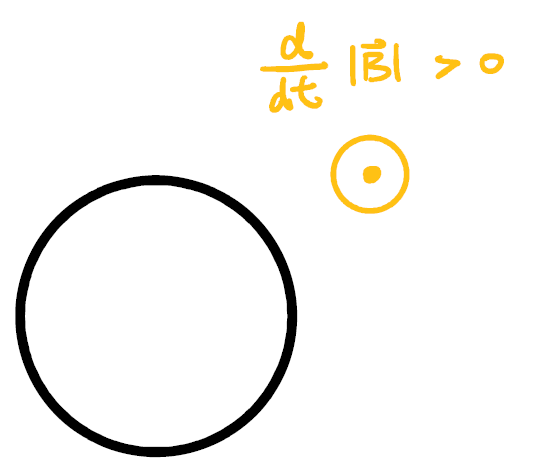
\includegraphics[height=6em]{lenz_eg1_1}
            \phantom{A}
        \end{minipage}
        {\huge \ $\Rightarrow$\ }
        \begin{minipage}{0.3\linewidth}
            \centering
            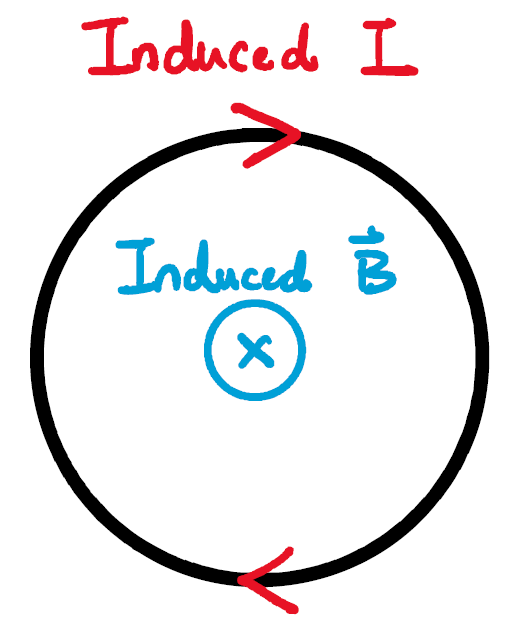
\includegraphics[height=6em]{lenz_eg1_2}
        \end{minipage}
    \end{center}

    \begin{enumerate}
        \item Magnetic flux is getting "more out-of-paper" due to 
        increase in B-field's magnitude.
        \item Induced EMF want to "oppose" this magnetic flux change.
        \item To oppose an increasing out-of-paper flux, one needs to decrease it,
        i.e. create an into-paper flux to compensate the increase.
        \item By right hand rule, into-paper flux can be created
        if a current flow clockwise in the ring. 
        So the induced EMF must be clockwise. 

    \end{enumerate}

    \begin{center}
        \begin{minipage}{0.75\linewidth}
            \centering
            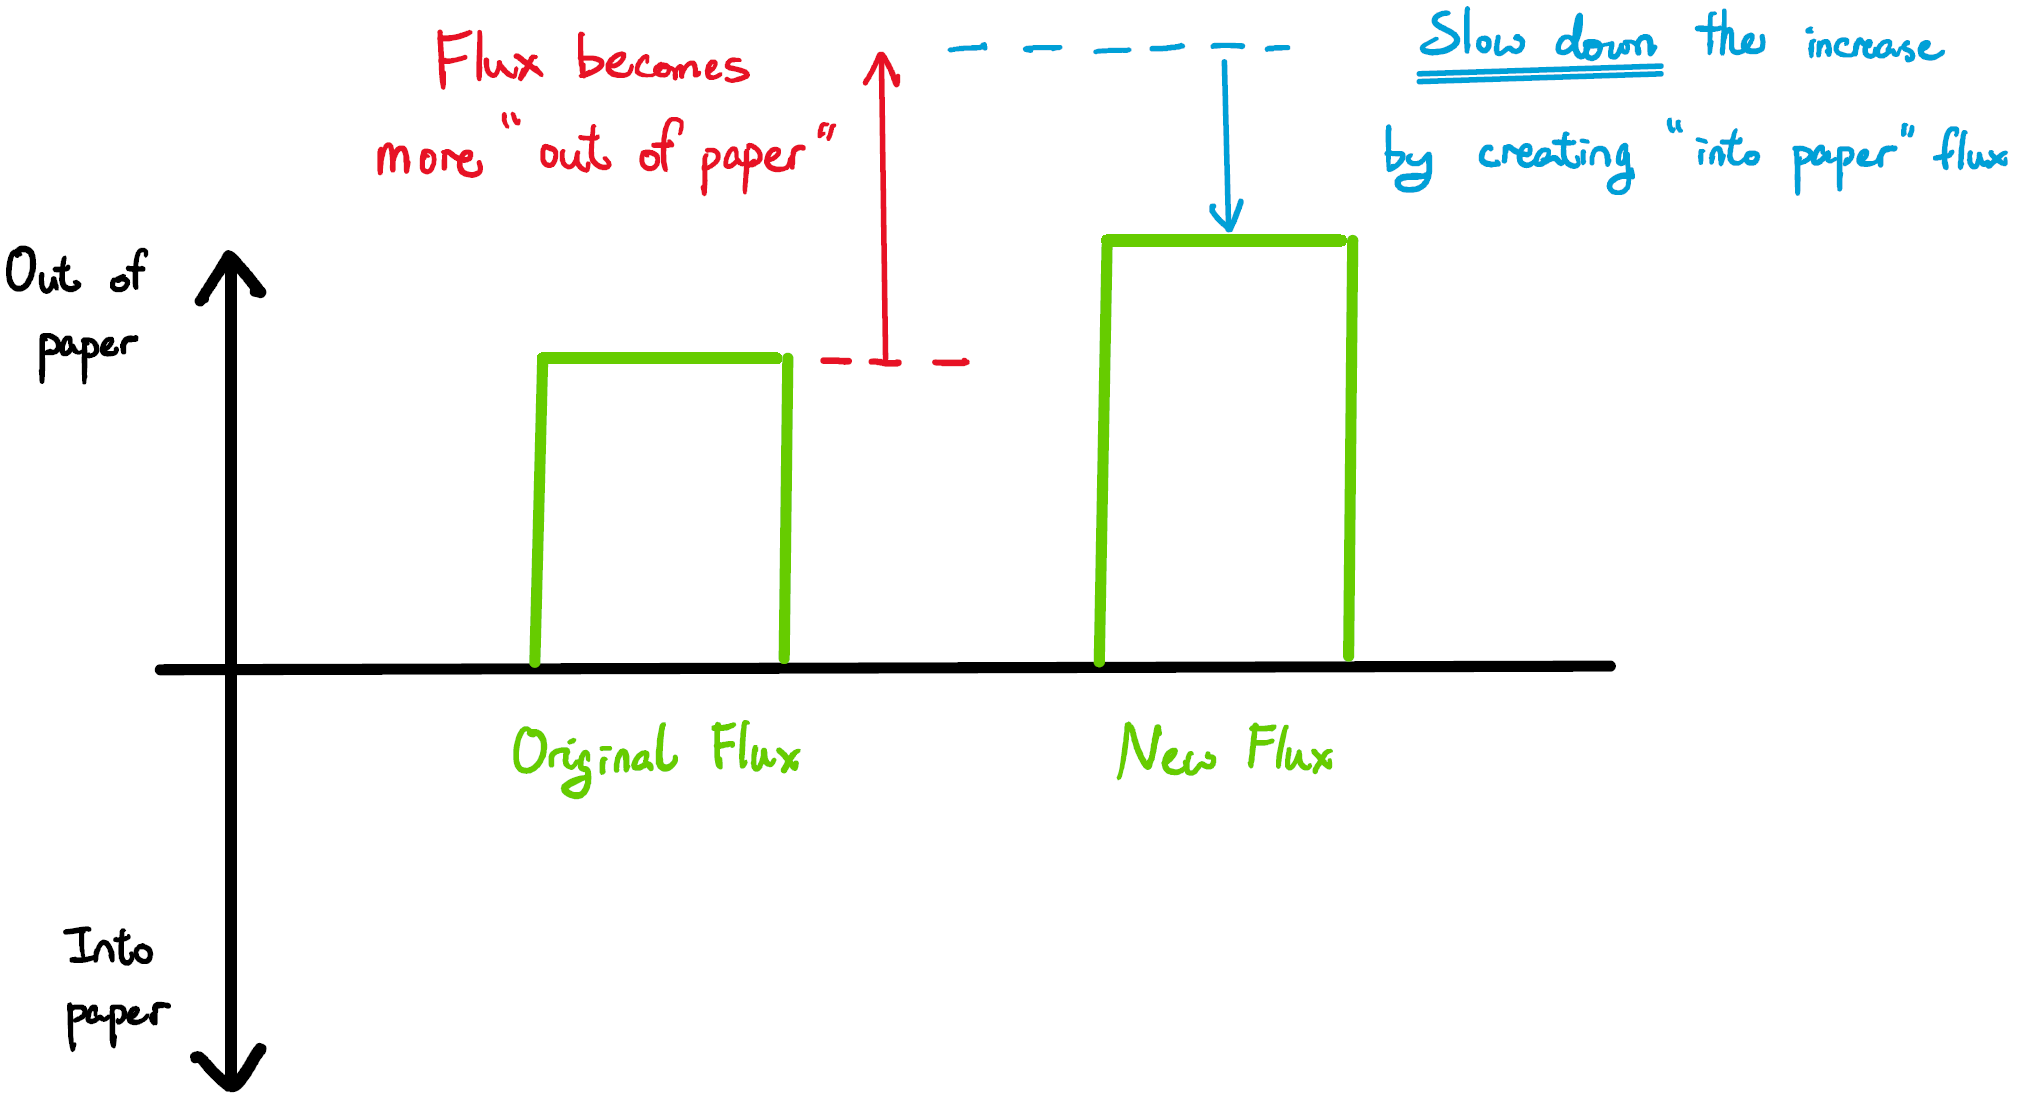
\includegraphics[width=\textwidth]{lenz_eg1_3}
        \end{minipage}
    \end{center}

\end{example}

\vskip 1ex
\begin{example}
    Consider a ring inside a constant into-paper B-field
    but is shrinking in radius.
    \begin{center}
        \begin{minipage}{0.3\linewidth}
            \centering
            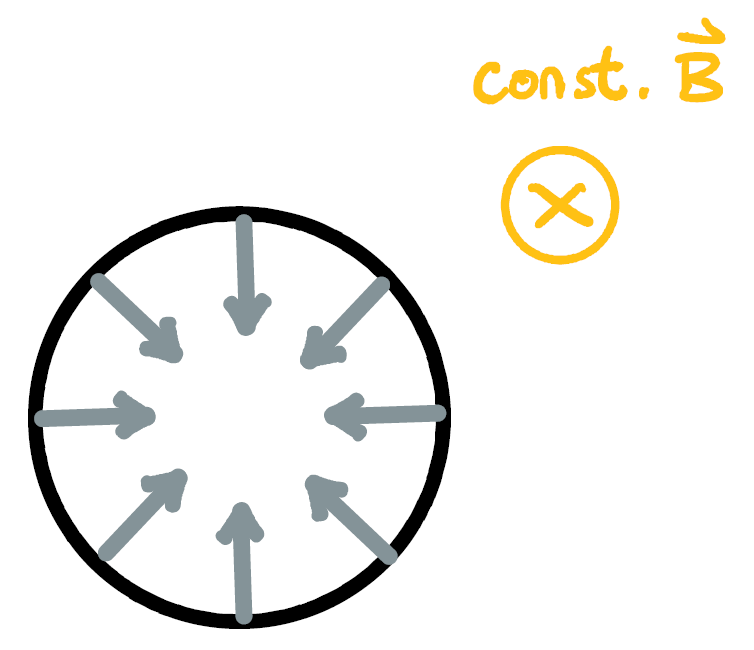
\includegraphics[height=6em]{lenz_eg2_1}
            \phantom{A}
        \end{minipage}
        {\huge \ $\Rightarrow$\ }
        \begin{minipage}{0.3\linewidth}
            \centering
            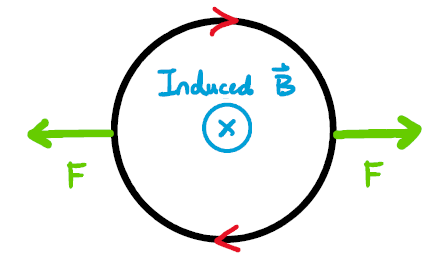
\includegraphics[height=6em]{lenz_eg2_2}
        \end{minipage}
    \end{center}

    \begin{enumerate}
        \item Magnetic flux is getting "less into-paper" due to
        decrease in area.
        \item Induced EMF want to "oppose" this magnetic flux change.
        \item To oppose a decreasing into-paper flux, one needs to increase it,
        i.e. create an into-paper flux to compensate the decrease.
        \item By right hand rule, into-paper flux can be created
        if a current flow clockwise in the ring.
        So the induced EMF must be clockwise.
        \item You can also notice that the forces on induced current 
        due to induced B field are pointing outward, 
        i.e. trying to stop the loop from contracting.
        
    \end{enumerate}

    \begin{center}
        \begin{minipage}{0.65\linewidth}
            \centering
            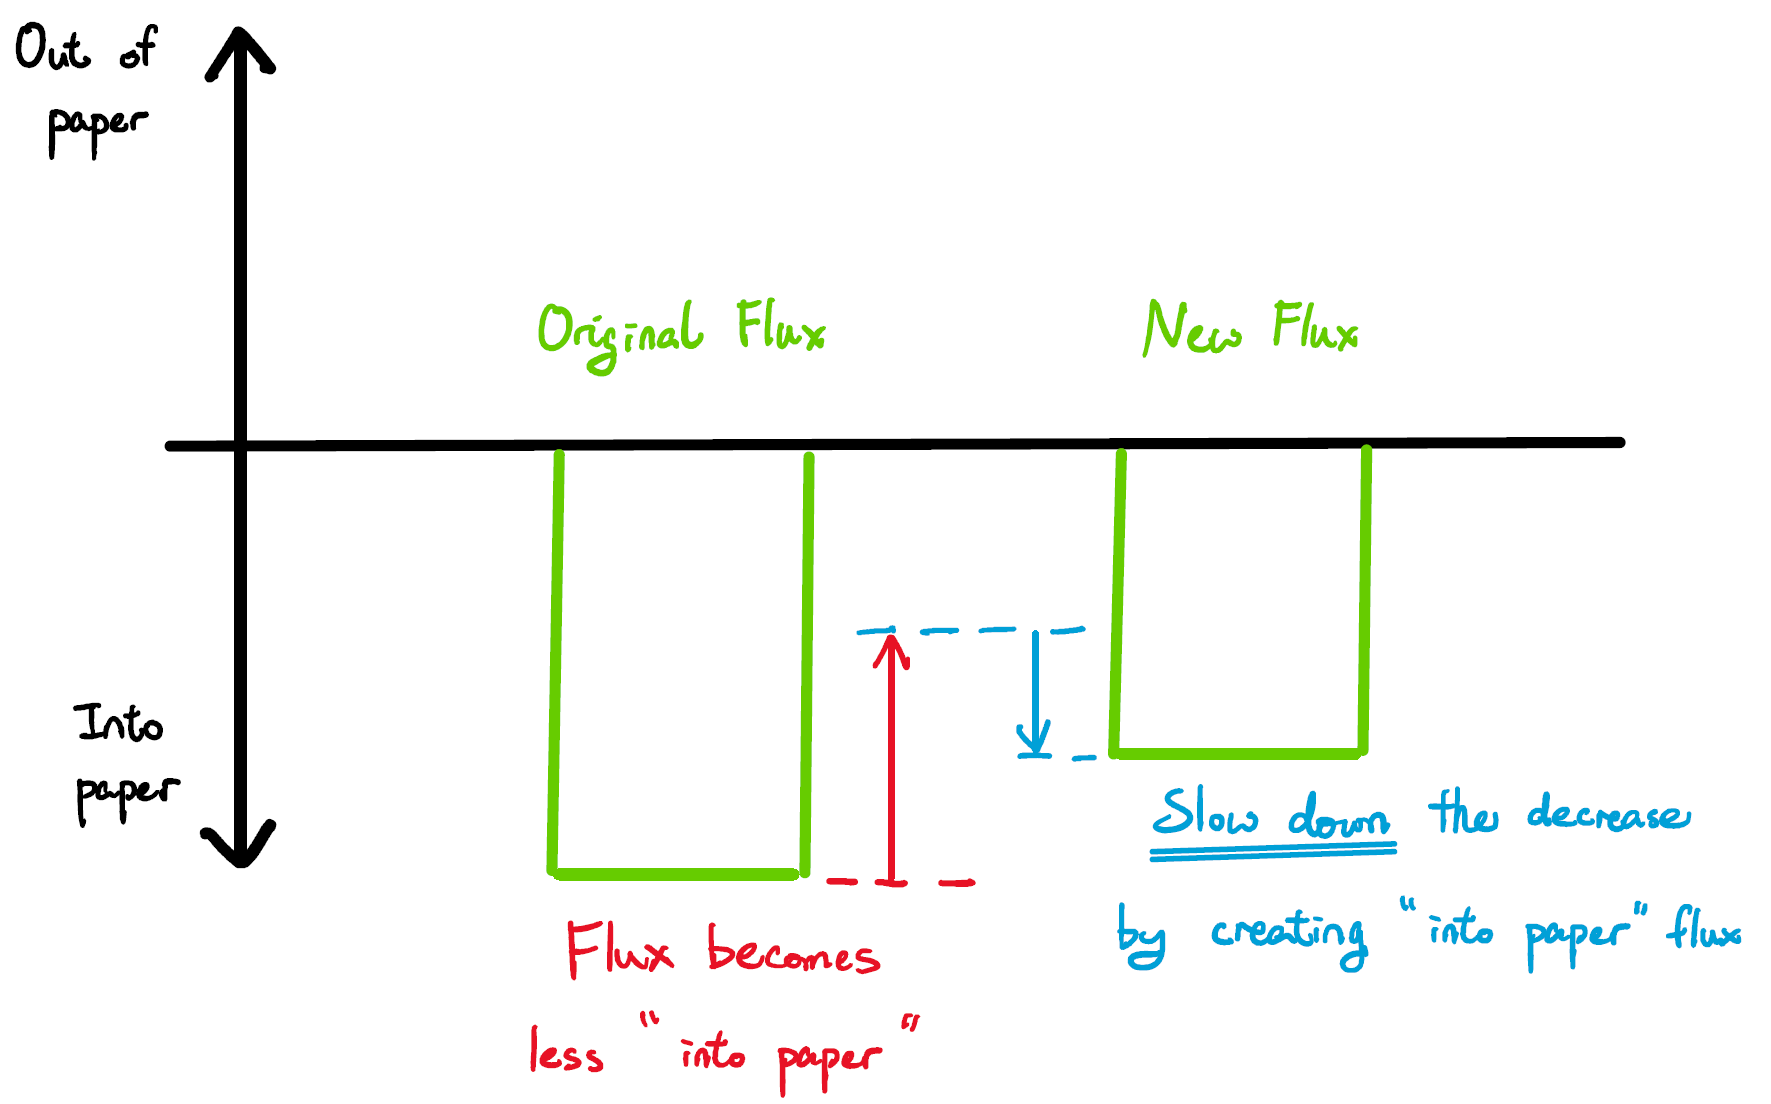
\includegraphics[width=\textwidth]{lenz_eg2_3}
        \end{minipage}
    \end{center}

\end{example}

\begin{notation}[Side note:]

    It may be tricky to see why induced EMF always wants to oppose the magnetic flux change,
    but it is quite easy to why the opposite cannot happen.\\

    Imagine if the EMF produces a magnetic flux that is in the same direction of the change 


\end{notation}


\linesep
% Section %%%%%%%%%%%%%%%%%%%%%%%%%%%%%%%%%%%%%%%%%%%%%%%%%%%%
\section{Solving Problems in Magnetic Induction}

Generally speaking, there are only two levels of questions related to magnetic induction.
\begin{itemize}
    \item Find EMF from the change in magnetic flux.
    \item Find induced E-field from the change in magnetic flux. 
\end{itemize}

The difference is in the difficulties - 
EMF is just a single number, the same everywhere in the coil.
But the E-field, when involving magnetic induction, 
is a vector function (distribution) that depends on position AND time.

%%%%%%%%%%%%
\subsection{Finding EMF}

This is a straightforward calculation to the surface integral of Faraday's law.

\begin{itemize}
    \item \bf{\ul{For high school level}} - 
    B-field is usually given as a constant of position,
    so that the surface integral reduces to a multiplication.
    \aleq{
        \epsilon = -\dvv{t}\iint \vvec{B}\cdot \dd{\vvec{s}}
        \ \sim\ -\dvv{t}\qty(\vvec{B}(t)\cdot \qty(\text{Area})(t))
    }

    And because you are not expected to have studied differentiation chain rule,
    you will never see a situation where both $\vvec{B}(t)$ and Area$(t)$ are changing.
    It is always given the rate of change of one of them and the other is fixed.
    \aleq{
        \cus[red]{\epsilon = -\vvec{B} \cdot \dvv{t}(\text{Area}(t))}
            {\substack{\text{When the question is about}\\\text{motional EMF}}}
        \qquad\text{or}\qquad
        \cus[red]{\epsilon = -\dvv{\vvec{B}(t)}{t} \cdot (\text{Area})}
            {\substack{\text{When the question is about}\\\text{transformer EMF}}}
    }

    \vskip 1ex
    \item \bf{\ul{For university level}} - You are assumed to have already learnt Ampere's law,
    so more likely you are given the current to find the B-field, before finding EMF. 
    \aleq{
        \text{First}\quad
        \cus[blue]{\oint \vvec{B}(t)\cdot\dd{\vvec{l}} = \mu_0 I(t)}{\text{Ampere's law for }\vvec{B}}
        \ ,\quad \text{then}\quad 
        \cus[blue]{\epsilon = -\dvv{t}\iint_{\text{Area}(t)} \vvec{B}(t)\cdot \dd{\vvec{s}}}{\text{Faraday's law for }\epsilon}
    }
\end{itemize}

And asking for the EMF's direction is pretty common,
because applying Lenz's law does not involve any maths.
All you need is your right hand.

%%%%%%%%%%%%
\subsection{Finding induced E-field}

This is in fact the task of solving the PDE of Maxwell-Faraday equation.
\aleq{
    \curl \vvec{E} = -\pdvv{\vvec{B}}{t}
    \qquad\Rightarrow\qquad
    \vvec{E}(t) = \text{Some function of }\vvec{B}(t)
}

Similar to how we deal with Gauss's law or Ampere's law,
we can avoid solving PDE in some very symmetrical cases.
If these conditions are satisfied:
\begin{enumerate}
    \item E-field is of the same magnitude everywhere on the loop.
    \item E-field make the same angle with each line segment of the loop.
\end{enumerate}

Then we can reduce the integral form of Maxwell-Faraday equation in to multiplication.
\aleq{
    -\dvv{t}\iint\vvec{B}\cdot\dd{\vec{s}} &= \oint \vvec{E}\cdot\dd{\vvec{l}}\\
    &= \oint \tkn{ampere_dot}{\cul[green]{\norm{\vvec{E}}\norm{\dd{\vvec{l}}}\cos\theta}}\\[1ex]
    &= \tkn{ampere_B}{\cul[red]{\norm{\vvec{E}}}}\ \tkn{ampere_theta}{\cul[blue]{\cos\theta}}\ \oint \norm{\dd{\vvec{l}}}\\[2.5em]
    &= \norm{\vvec{E}}\ \cos\theta\ (\text{Perimeter of loop})\\[1em]
    \Aboxed{
        \norm{\vvec{E}} &= \frac{\dvv{t}\qty(\text{Flux of }\vvec{B})}{(\text{Perimeter of loop})\cos\theta}
    }
}
\addArrow[green]{ampere_dot}{(5ex,0)}
{\scriptsize Just dot product\\[-1ex]\scriptsize $\vvec{a}\cdot\vvec{b}=\norm{\vvec{a}}\norm{\vvec{b}}\cos\theta$}
{(8ex,0)}{(6ex,0)}
\addBentArrow[red]{ampere_B}{(-8ex,-3.5ex)}
{Same magnitude everywhere\\[-0.5ex]Can move out of integral!}
{(0,-1.5ex)}{(-12.5ex,1ex)}
\addBentArrow[blue]{ampere_theta}{(8ex,-3.5ex)}
{Form same angle everywhere\\[-0.5ex]Can move out of integral!}
{(0,-1.5ex)}{(12.5ex,1ex)}

\begin{example}
    Consider a static rectangular loop next to an infinitely long wire, 
    which carries a time-varying current $I(t)$, same magnitude everywhere along the wire. 

    \begin{center}
        \begin{minipage}{0.3\linewidth}
            \centering
            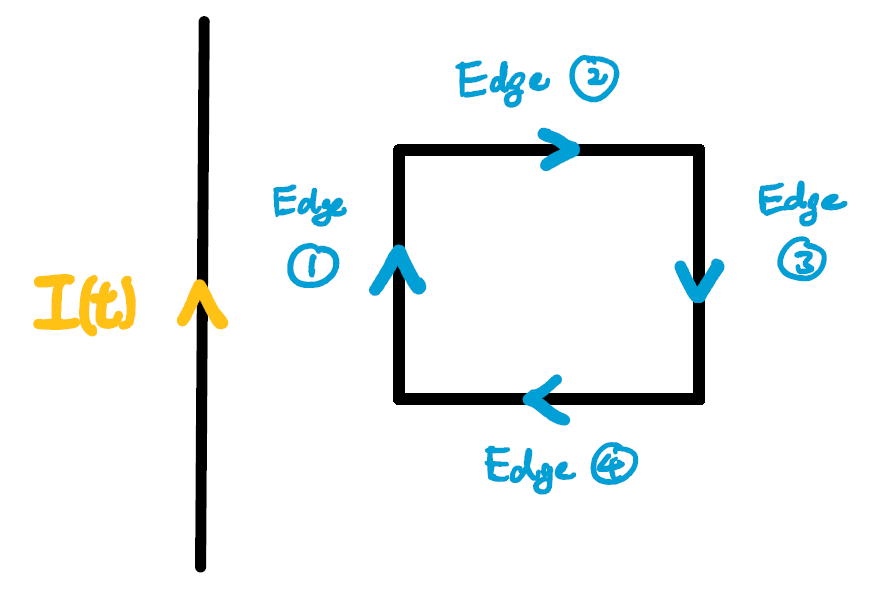
\includegraphics[width=\textwidth]{frame1}
        \end{minipage}
    \end{center}

    \begin{enumerate}
        \item Always start with finding the magnetic flux through the loop.
        By Ampere's law, the B-field by an infinitely long wire is 
        \aleq{
            \vvec{B}(r,t) = \frac{\mu_0}{2\pi}\frac{I(t)}{r}
        }
        
        The magnetic flux through the loop can be calculated by 
        first dividing the loop's area into strips,
        then integrate the flux of all strips.

        \begin{minipage}{0.6\linewidth}
            \aleq{
                \Phi_B &= \iint \vvec{B}\cdot\dd{\vvec{s}}\\
                &= \int_{r_1}^{r_2} \frac{\mu_0 I(t)}{2\pi r} (L\dd{r})\\
                &= \frac{\mu_0 I(t) L}{2\pi}\qty[\ln(r_2)-\ln(r_1)]
            }
        \end{minipage}
        \hspace{0.05\textwidth}
        \begin{minipage}{0.3\linewidth}
            \centering
            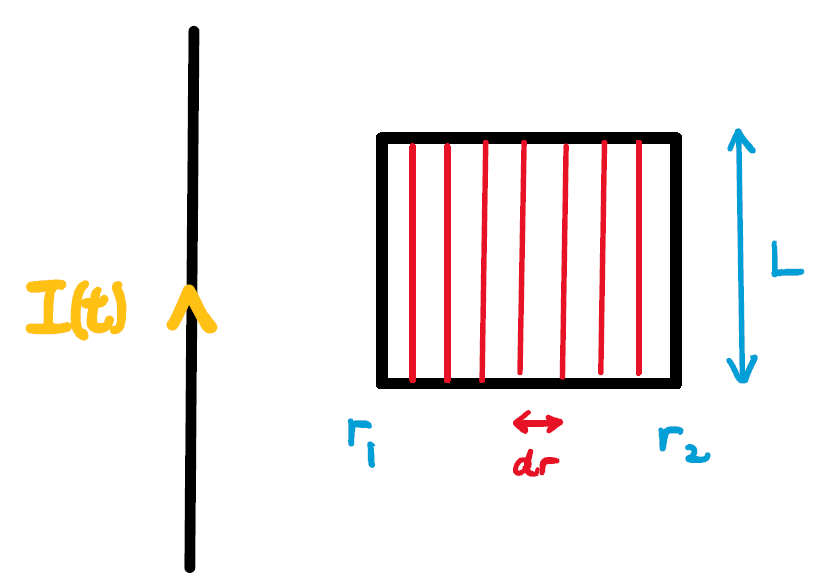
\includegraphics[width=\textwidth]{frame2}
        \end{minipage}
        
        \vskip 1em
        \item The total EMF generated in the loop is just the differentiation of the above. i.e.
        \aleq{
            \epsilon = \frac{\mu_0 L}{2\pi}\qty(\dvv{I(t)}{t})[\ln(r_2) - \ln(r_1)]
        }
        Direction of the EMF depends on how the current varies.
        For example, if $\dv{I(t)}{t}>0$, i.e. magnetic flux increasing in the into-paper direction.
        To oppose the change, EMF must be in anti-clockwise direction
        to produce an out-of-paper direction flux.

        \vskip 1em
        \item On the other hand, to compute the E-field distribution, all we only know is 
        
        \begin{minipage}{0.6\linewidth}
            \aleq{
                \abs{\epsilon} &= \oint \vvec{E}\cdot \dd{\vvec{l}} \\
                &= E^{\parallel}_1 L + E^{\parallel}_2 (r_2-r_1) + E^{\parallel}_3 L + E^{\parallel}_4 (r_2-r_1)
            }
        \end{minipage}
        \hspace{0.05\textwidth}
        \begin{minipage}{0.3\linewidth}
            \centering
            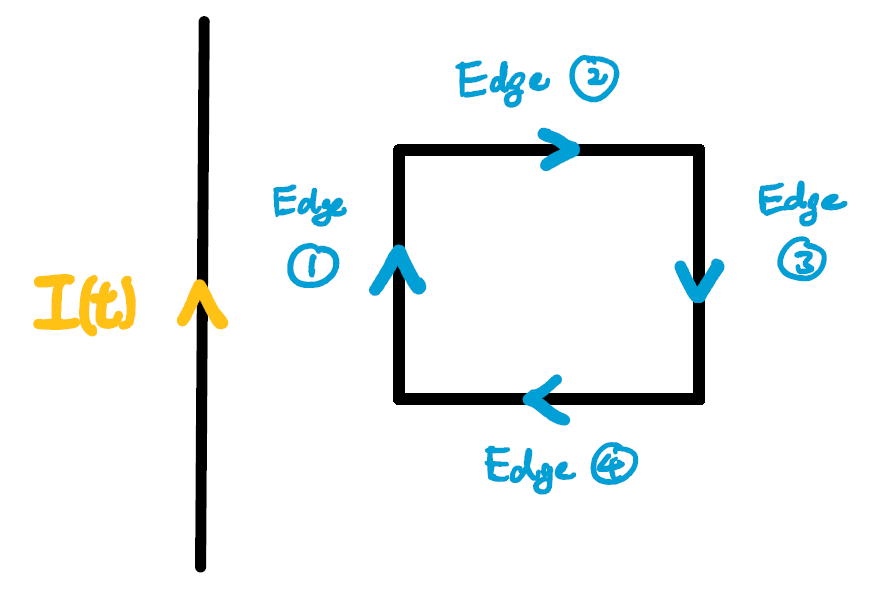
\includegraphics[width=\textwidth]{frame3}
        \end{minipage}

        Note that after taking dot product, only the component parallel to the edge is left.\\

        To find the $E$ on each edge, we need symmetry arguments.
        \begin{itemize}
            \item By translational symmetry along the wire, 
            $E_2^\parallel$ and $E_4^\parallel$ must be the same. 
            Their contributions of dot product along the loop are cancelled.

            \item By rotation symmetry about the wire, 
            the E-field is only a function of radial distance from the wire. 
            We can claim that $E^\parallel_1$ and $E^\parallel_3$ must have the same function form $E^\parallel(r)$,
            
            \begin{center}
                \begin{minipage}{0.4\linewidth}
                    \centering
                    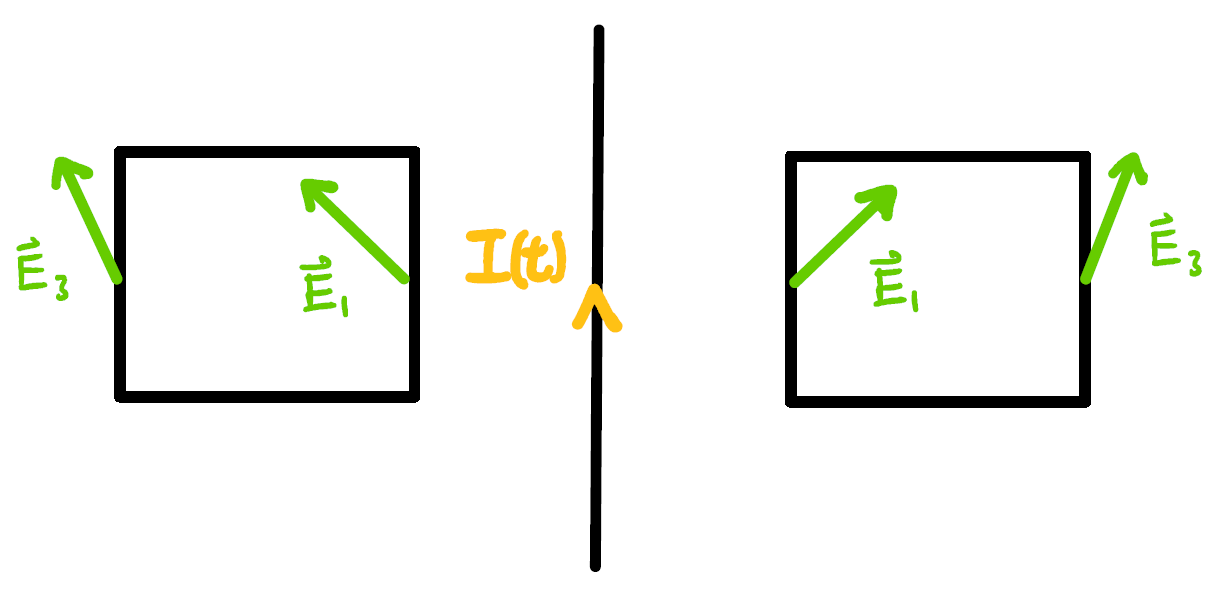
\includegraphics[width=\textwidth]{frame4}
                \end{minipage}
            \end{center}
            
        \end{itemize}
        
        So the E-field relation to EMF is reduced to
        \aleq{
            \abs{\epsilon} &= E^{\parallel}_3 L - E^{\parallel}_1 L \\[1ex]
            &= E^{\parallel}(r_2) L - E^{\parallel}(r_1) L\\[1ex]
            &\equiv \frac{\mu_0 L}{2\pi}\qty(\dvv{I(t)}{t}) \qty[\ln(r_2)-\ln(r_1)]
        }
        
        Therefore we can claim that \cul[red]{$\vvec{E}$ 's component parallel to the wire} is
        \aleq{
            E^{\parallel}(r) = \frac{\mu_0}{2\pi}\qty(\dvv{I(t)}{t})\ln(r)
        }

        \newpage
        \item Note that in the above analysis,
        we cannot determine if the E-field has components perpendicular to the wire.

        \begin{center}
            \begin{minipage}{0.3\linewidth}
                \centering
                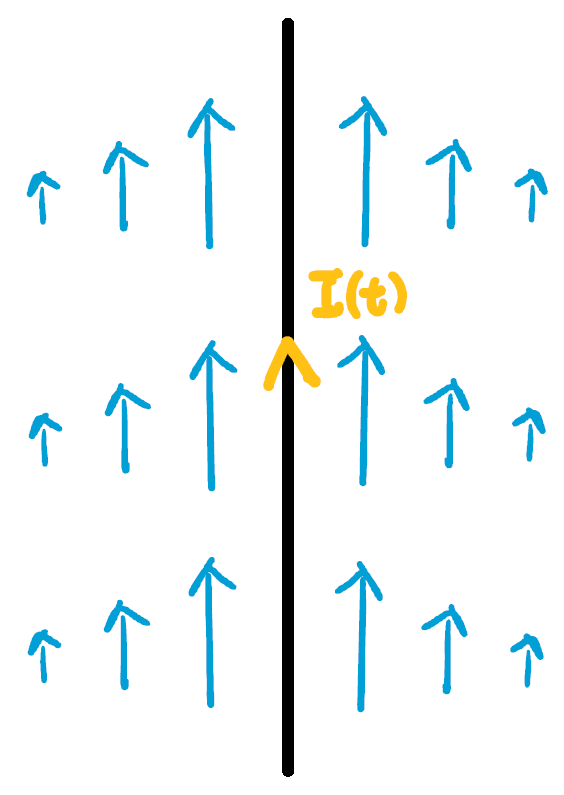
\includegraphics[height=10em]{field1}\\
                If the field only has component parallel\\ to the wire
            \end{minipage}
            \hspace{0.05\textwidth}
            \begin{minipage}{0.3\linewidth}
                \centering
                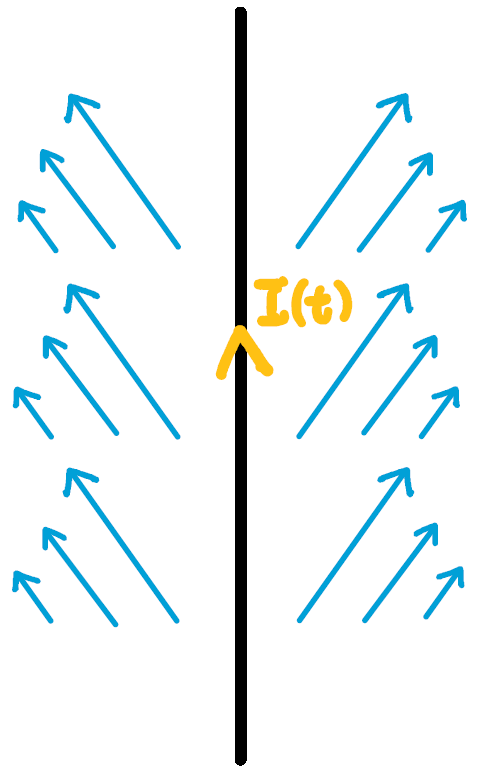
\includegraphics[height=10em]{field2}\\
                If the field has both components parallel and normal to the wire
            \end{minipage}
        \end{center}
        
        Recall from Gauss's law, 
        E-field can be perpendicular to the wire if the wire carries a \cul[red]{static} line charge density.
        So when the wire carries BOTH net charge and time-varying current,
        the total E-field will be in diagonal directions.

        \begin{center}
            \begin{minipage}{0.2\linewidth}
                \centering
                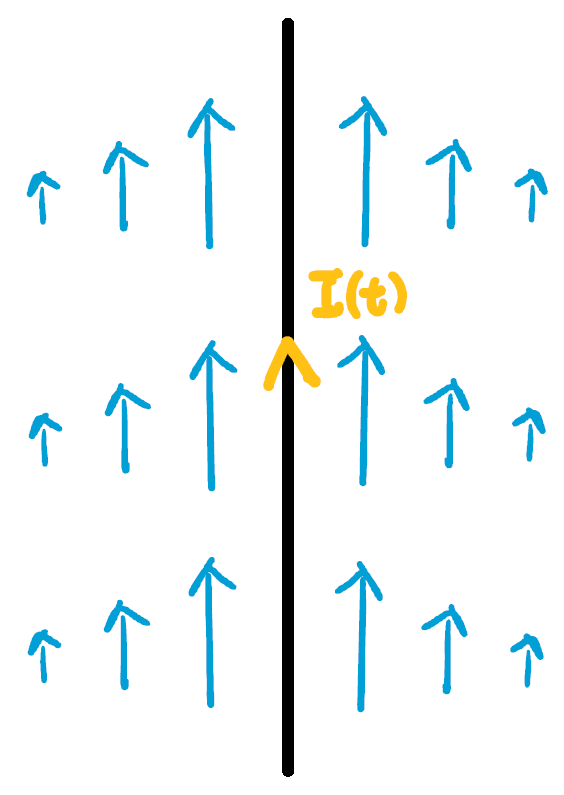
\includegraphics[height=10em]{field1}
            \end{minipage}
            {\huge \quad$+$\quad}
            \begin{minipage}{0.2\linewidth}
                \centering
                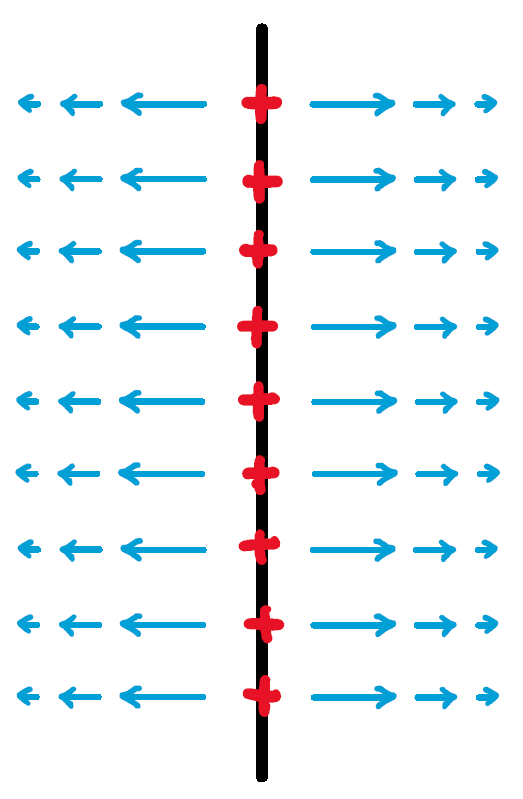
\includegraphics[height=10em]{field3}
            \end{minipage}
            {\huge \quad$=$\quad}
            \begin{minipage}{0.2\linewidth}
                \centering
                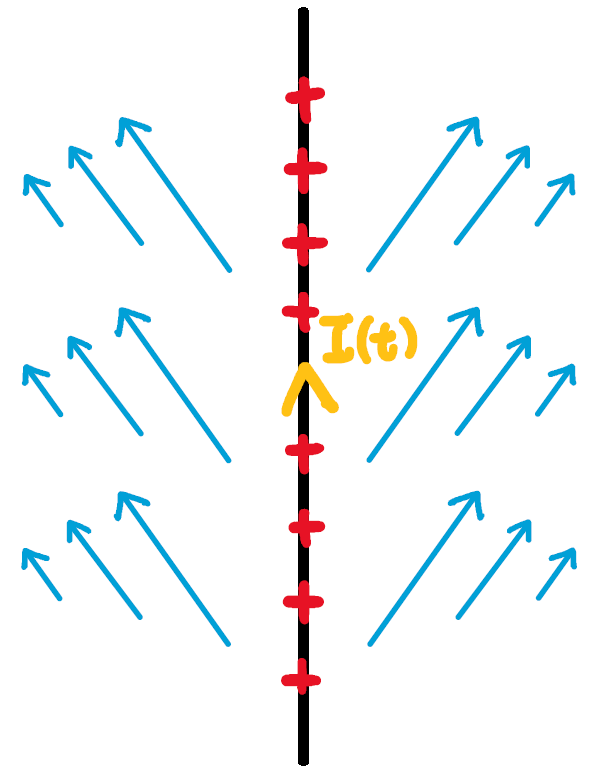
\includegraphics[height=10em]{field4}
            \end{minipage}
        \end{center}

    \end{enumerate}

    
\end{example}


\theend

\newpage
\appendix
% Section %%%%%%%%%%%%%%%%%%%%%%%%%%%%%%%%%%%%%%%%%%%%%%%%%%%%
%\setcounter{section}{-1}
\section*{Appendix: A Brief History of Electromagnetism}

Contents under magnetic induction may seem unorganized because of its developments:
\begin{itemize}
    \item The phenomena was discovered very early in 1830s.
    \item The first time it was formulated rigorously in maths, was 30 years later.
    \item The modern explanation we used - Lorentz force, was formulated 60 years later.
\end{itemize}

For your reference, 
here lists the most important advancements in the history of E\&M.

\begin{center}
    \begin{tabularx}{\textwidth}{
        >{\centering\arraybackslash}m{0.15\textwidth} 
        p{0.8\textwidth}
        }

        Year & \makecell[c]{Advancement} \\ 
        \hline
        Before 1500s & 
        Different electrostatics phenomena were known.
        But they were not unified or explained at all. \\
        %
        1600 &
        \makecell[tl]{
            \href{https://en.wikipedia.org/wiki/William_Gilbert_(physicist)}{William Gilbert}
            was the first person to use the word "electrical" to describe\\ electrostatics phenomena. 
            Also the first to propose that electrical effect is\\ due to flows of particles.
        }\\[1.5em]
        %
        1750 &
        \makecell[tl]{
            \href{https://en.wikipedia.org/wiki/Benjamin_Franklin}{Benjamin Franklin} 
            developed a one "fluid" theory of electricity, 
            and called\\ this fluid "charge".
        }\\[1.5em]
        %
        1784 &
        \makecell[tl]{
            \href{https://en.wikipedia.org/wiki/Charles-Augustin_de_Coulomb}{Charles-Augustin de Coulomb}
            experimentally showed that force between\\ charged objects $\propto \inv{r^2}$.
            \gray{(Coulomb's law $F = \inv{4\pi\epsilon_0}\frac{Qq}{r^2}$)}
        }\\[1.5em]
        %
        1800 &
        \makecell[tl]{
            \href{https://en.wikipedia.org/wiki/Alessandro_Volta}{Alessandro Volta}
            Made the first battery from electro-chemistry.\\
            \gray{(First time to have steady current.)}
        }\\[1.5em]
        %
        1820 &
        \makecell[tl]{
            \href{https://en.wikipedia.org/wiki/Hans_Christian_\%C3\%98rsted}{Hans Christian Ørsted}
            discovered that current wire can deflect compress.\\
            \gray{(First time to relate electric and magnetic phenomena.)}
        }\\[2em]
        %
        1820 &
        \makecell[tl]{
            \href{https://en.wikipedia.org/wiki/Andr\%C3\%A9-Marie_Amp\%C3\%A8re}{André-Marie Ampère}
            formulated and verified the force between current wires.\\
            \gray{$(F = I\vvec{l}_1\cross \frac{\mu_0 I}{2\pi r}\vvec{l}_2)$}
        }\\[2em]
        %
        1831 &
        \makecell[tl]{
            \href{https://en.wikipedia.org/wiki/Michael_Faraday}{Michael Faraday}
            discovered phenomena of magnetic induction - induced EMF\\
            can be generated in two ways: Motional EMF and transformer EMF.
        }\\[1.5em]
        %
        1834 &
        \makecell[tl]{
            \href{https://en.wikipedia.org/wiki/Emil_Lenz}{Emil Lenz}
            Explained direction of induced current by energy conservation.\\
            \gray{(Lenz's Law)}
        }\\[1.5em]
        %
        1860 &
        \makecell[tl]{
            \href{https://en.wikipedia.org/wiki/James_Clerk_Maxwell}{James Clerk Maxwell}
            unified past discoveries into 20 equations, 
            and used\\ field description for the first time.\\[0.5ex]
            \bf{\ul{$\ast\ast\ast$ This was the first time $\vvec{E}$ and $\vvec{B}$ appeared as field. $\ast\ast\ast$}}\\
            \bf{Before Maxwell, everything was described in terms of force.}
        }\\[4em]
        %
        1893 &
        \makecell[tl]{
            \href{https://en.wikipedia.org/wiki/Oliver_Heaviside}{Oliver Heaviside}
            combined Maxwell's 20 equations into 4, by vector calculus.\\
            \gray{(This is the version of Maxwell's equation we now know.)}
        }\\[1em]
        %
        1895 &
        \makecell[tl]{
            \href{https://en.wikipedia.org/wiki/Hendrik_Lorentz}{Hendrik Lorentz}
            derive the correct force on charges under both $\vvec{E}$ and $\vvec{B}$.\\
            \gray{(Lorentz force formula)}
        }\\[1em]
        %
        After 1900s &
        Entering the relativistic and quantum era. Not classical E\&M anymore. \\

    \end{tabularx}
\end{center}


%%%

\end{document}